\chapter{Implementacija i korisničko sučelje}


\section{Korištene tehnologije i alati}

\noindent Za komunikaciju tima korištene su aplikacije \underline{WhatsApp}\footnote{https://www.whatsapp.com/} i \underline{Discord}\footnote{https://discord.com}. Za izradu UML dijagrama korišten je \underline{Astah Professional}\footnote{http://astah.net/editions/professional}.

Za izradu dokumentacije korišten je \underline{LaTeX}\footnote{https://www.latex-project.org}, sustav za izradu dokumenata koji koristi markup jezik. Za upravljanje izvornim kodom korišten je \underline{Git}\footnote{https://git-scm.com/}. Repozitorij projekta dostupan je na platformi \underline{GitHub}\footnote{https://github.com}.

Za razvojna okruženja korišteni su \underline{Visual Studio Code}\footnote{https://visualstudio.microsoft.com/}. Visual Studio Code je integrirano razvojno okruženje (IDE) kompanije Microsoft. Koristi se za razvoj wen-stranica, web-aplikacija, web-usluga i mobilnih aplikacija. Za razvoj softvera koristi Windows API, Windows Forms, Windows Presentation Foundation, Windows Store i Microsoft Silverlight.

Za pisanje aplikacije korišten je \underline{Spring Boot}\footnote{https://spring.io/projects/spring-boot/}, framework za razvoj Java aplikacija, za razvoj backenda. Za razvoj frontenda korišten je \underline{React}\footnote{https://react.dev}, biblioteka za izgradnju sučelja u jeziku \underline{JavaScript}\footnote{https://www.javascript.com/}. Također je korišten \underline{TypeScript}\footnote{https://www.typescriptlang.org} kao nadogradnja nad JavaScriptom. On poboljšava kvalitetu i održivost koda napisanog u JavaScriptu. U pogledu korisničkog sučelja, integrirana je i \underline{Ant Design}\footnote{https://ant.design/}, popularna biblioteka za React koja pruža širok spektar već gotovih komponenata. Ant Design je korišten za implementaciju određenih dijelova korisničkog sučelja kako bi se postigla dosljednost i funkcionalnost.


Baza podataka nalazi se na poslužitelju 

\eject


\section{Ispitivanje programskog rješenja}

%\textbf{\textit{dio 2. revizije}}\\

%\textit{U ovom poglavlju je potrebno opisati provedbu ispitivanja implementiranih funkcionalnosti na razini komponenti i na razini cijelog sustava s prikazom odabranih ispitnih slučajeva. Studenti trebaju ispitati temeljnu funkcionalnost i rubne uvjete.}


\subsection{Ispitivanje komponenti}
U procesu testiranja funkcionalnosti komponenti,  koristili smo popularni radni okvir \textit{JUnit}. Kako bi testiranje bilo izolirano, potrebno je simulirati komponente o kojima ovisi komponenta koju testiramo. U tu svrhu smo koristili programski okvir \textit{Mockito}. Ukupno smo implementirali sedam testirajućih metoda unutar tri testirajuće klase.

\vspace{1em}

U svrhu testiranja funkcionalnosti klase \textit{KorisnikController}, implementirali smo tri metode. Specifično, testirajuća metoda \ref{fig:test1} ima za cilj provjeriti ispravnost metode za registraciju novog korisnika kada su joj proslijeđeni valjani podaci za registraciju (ime, prezime, korisničko ime, lozinka, e-mail i uloga) te slika profila. Očekujemo da će rezultat testirane metode biti objekt tipa \textit{Korisnik}, koji će sadržavati točne podatke (prethodno proslijeđene) o novostvorenom korisniku.

\begin{figure}[H]
	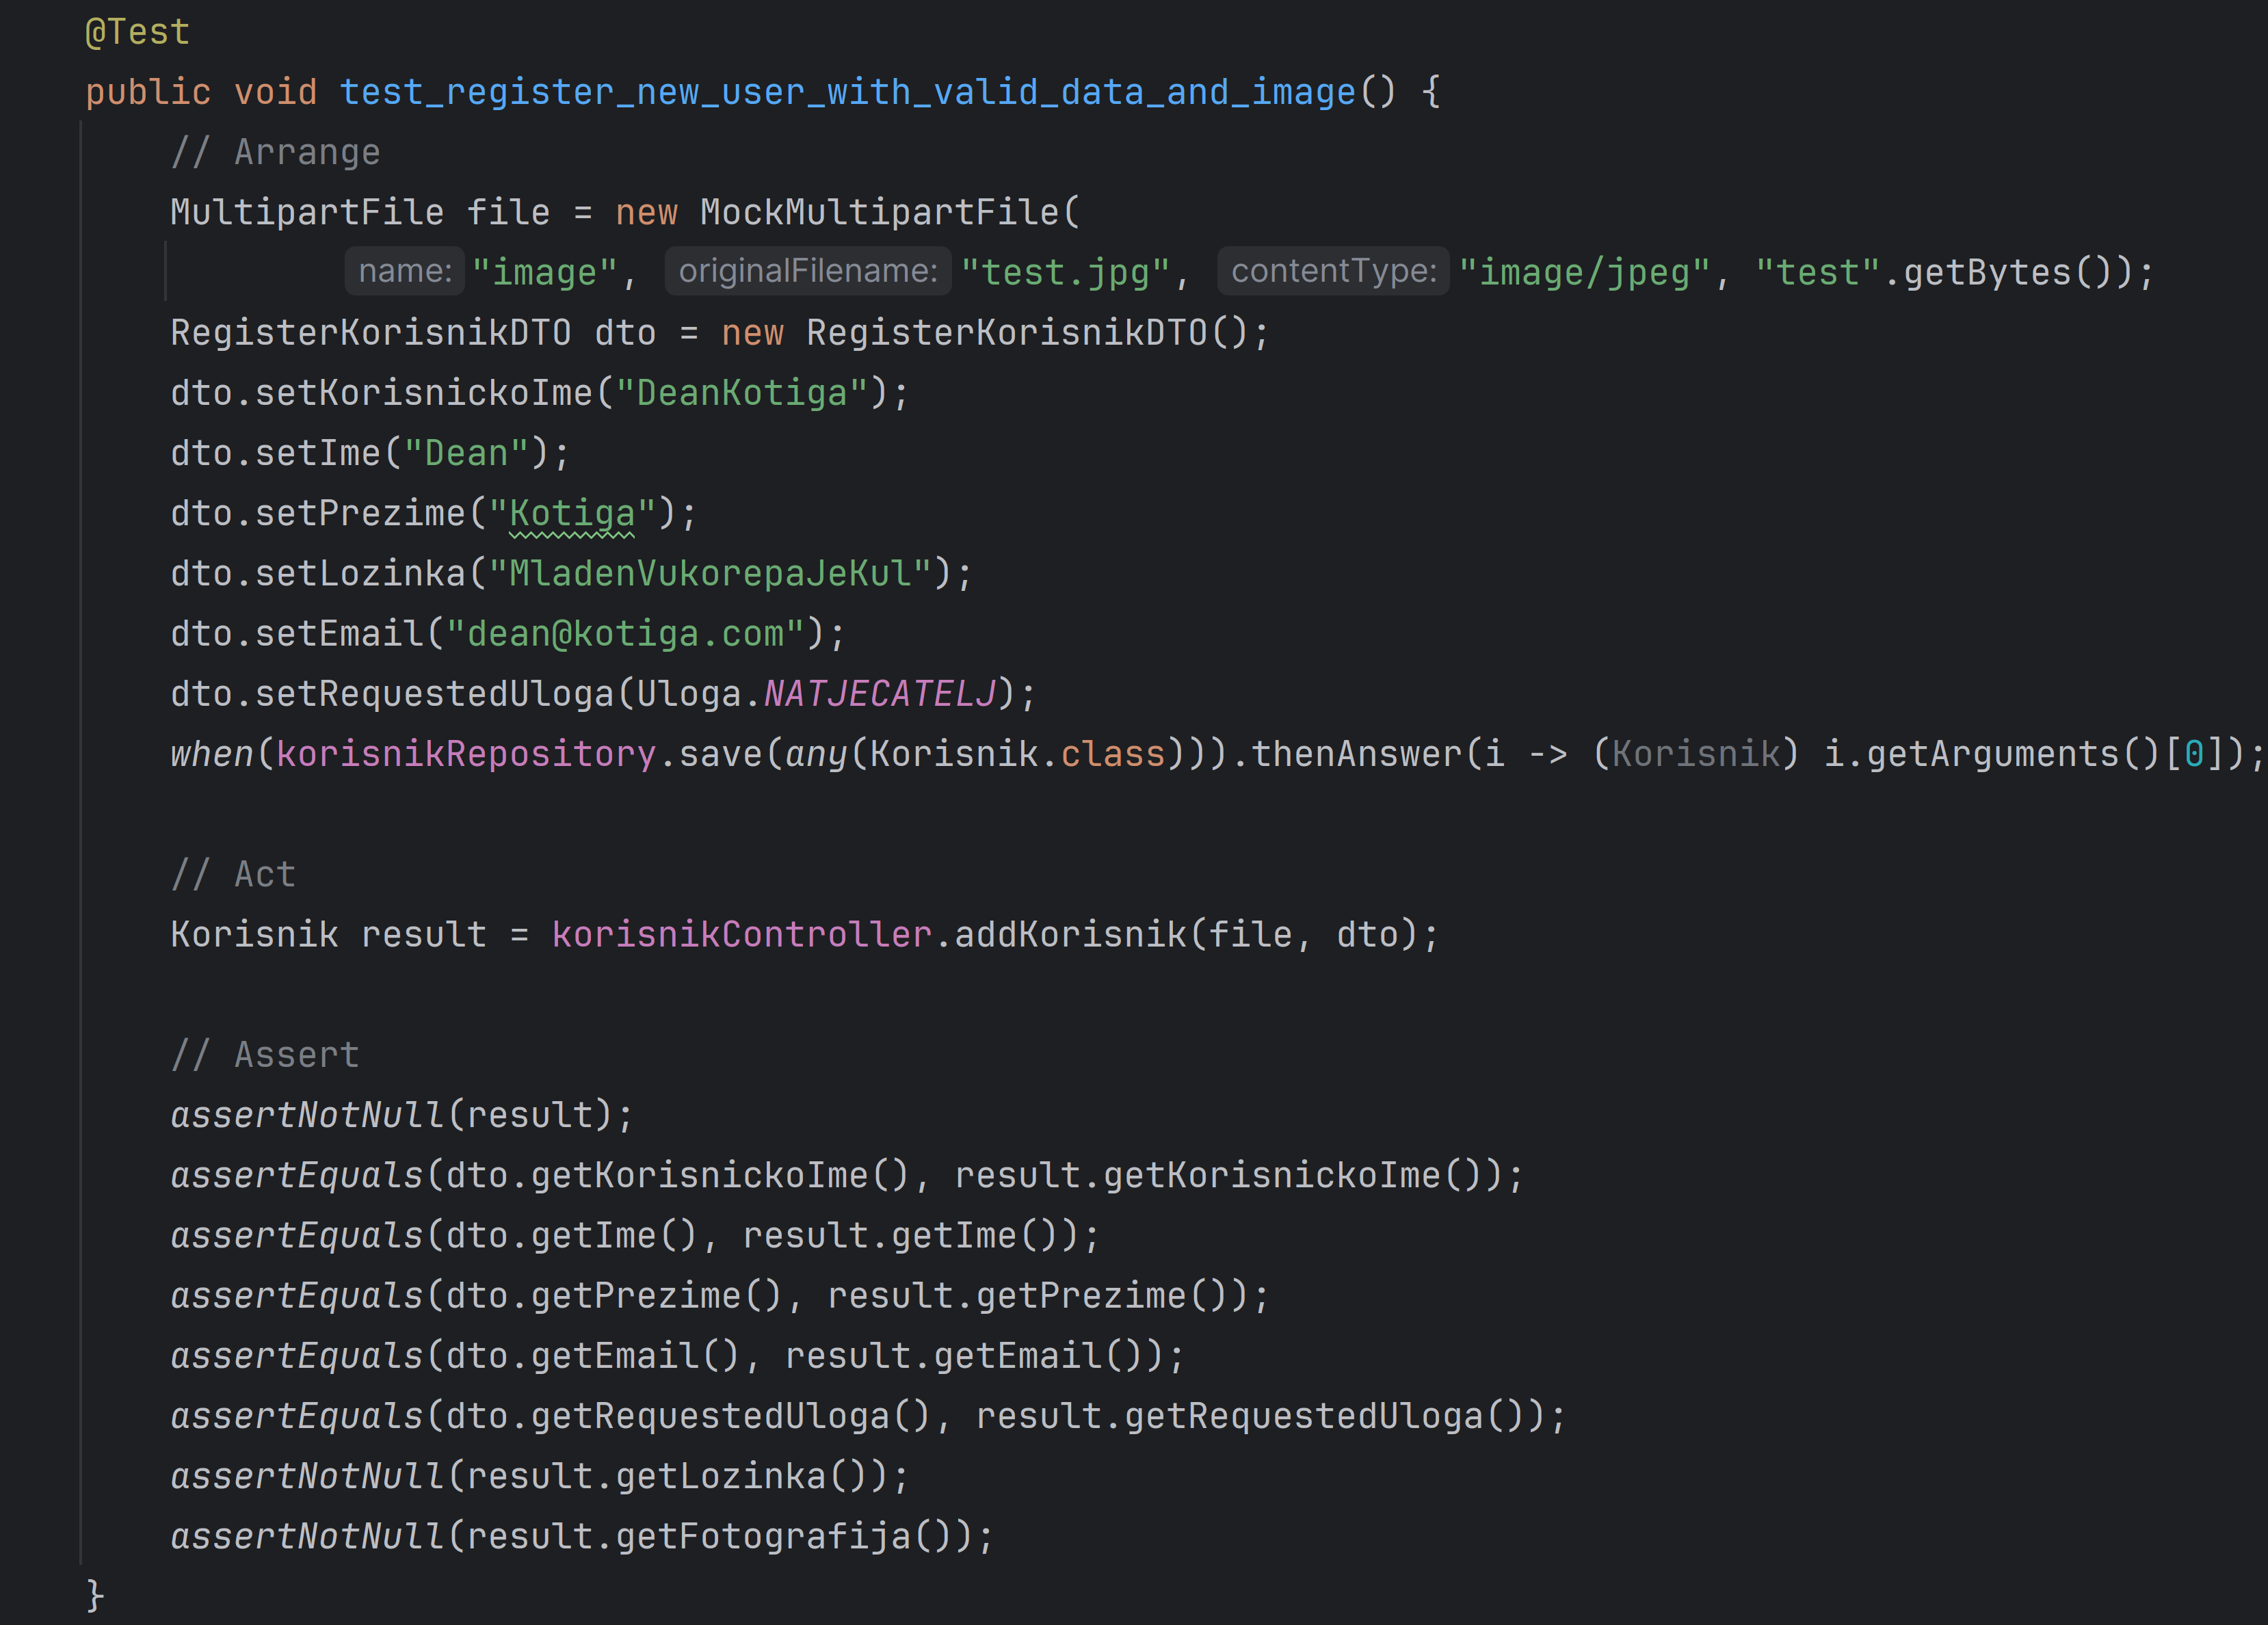
\includegraphics[scale=0.15]{slike/test1.png}
	\centering
	\caption{Testirajuća metoda - registracija korisnika}
	\label{fig:test1}
\end{figure}

Za razliku od prethodne, testirajuća metoda \ref{fig:test2} provjerava ispravnost iste metode u situaciji kada se pokuša dodati korisnik s korisničkim imenom koje je već zauzeto.  U ovome ispitnom slučaju se očekuje da će testirana metoda prepoznati ovu situaciju i shodno tome baciti očekivanu iznimku.

\begin{figure}[H]
	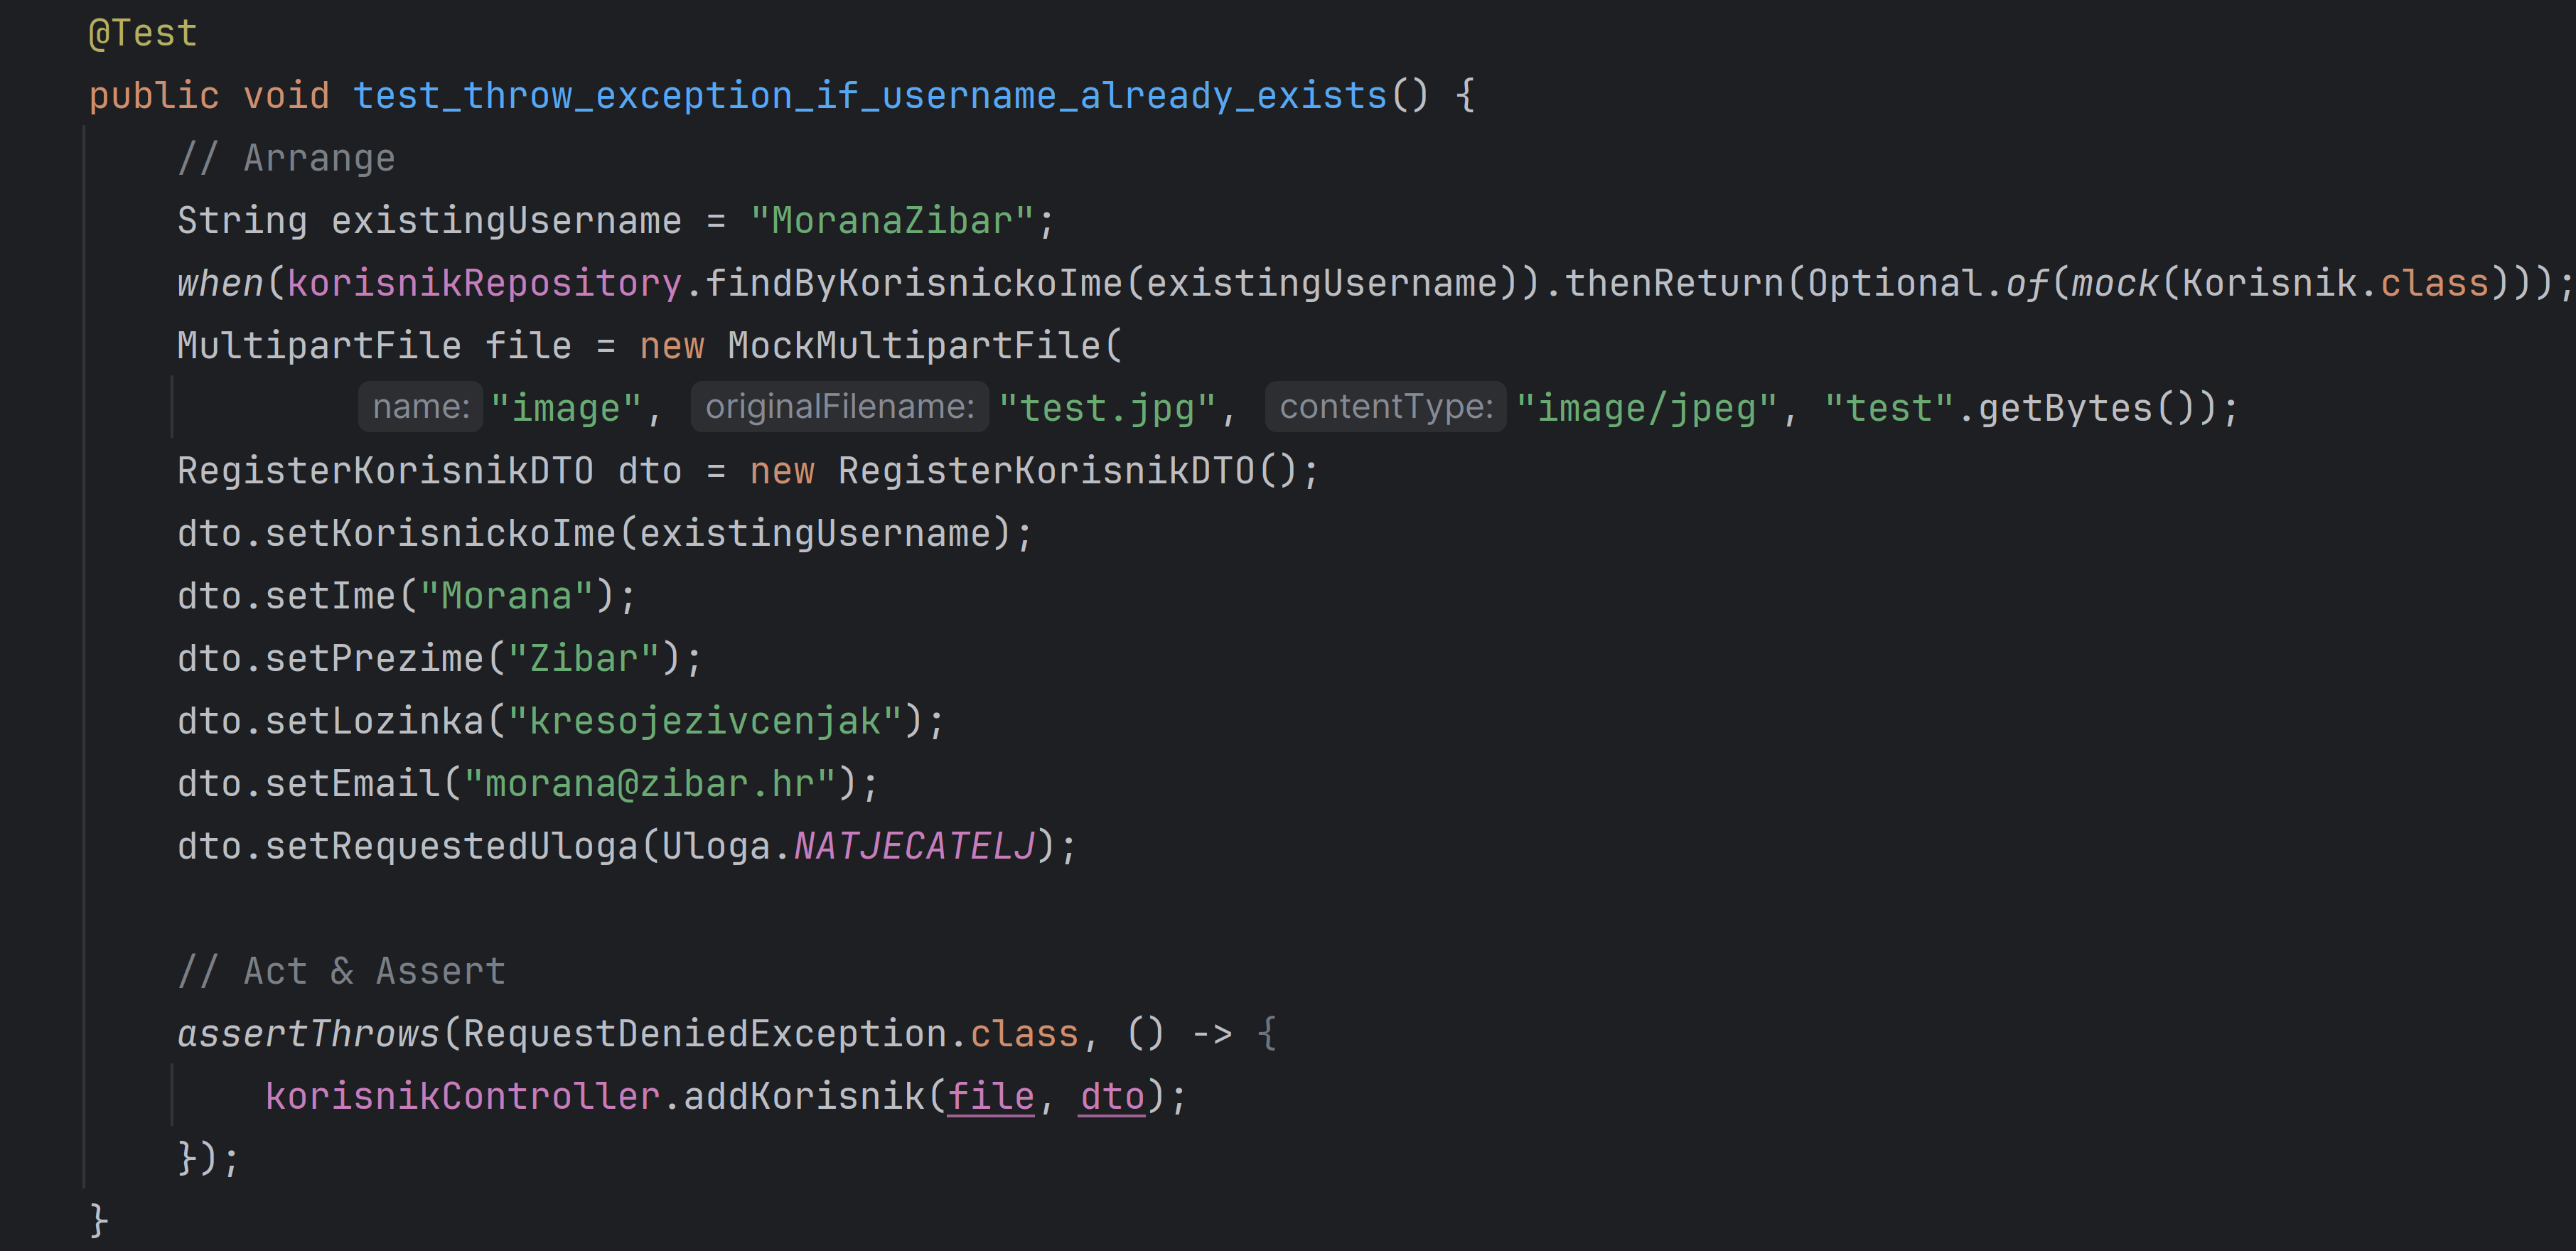
\includegraphics[scale=0.15]{slike/test2.png}
	\centering
	\caption{Testirajuća metoda - neuspješna registracija korisnika}
	\label{fig:test2}
\end{figure}

Posljednjim ispitnim slučajem \ref{fig:test3} za klasu \textit{KorisnikController} želimo verificirati  ispravnost metode za potvrdu zahtijevanih uloga korisnika od strane administratora. Očekuje se da će nakon uspješne potvrde testirana metoda, koja kao argument prima korisničko ime, vratiti HTTP odgovor sa statusom OK.

\begin{figure}[H]
	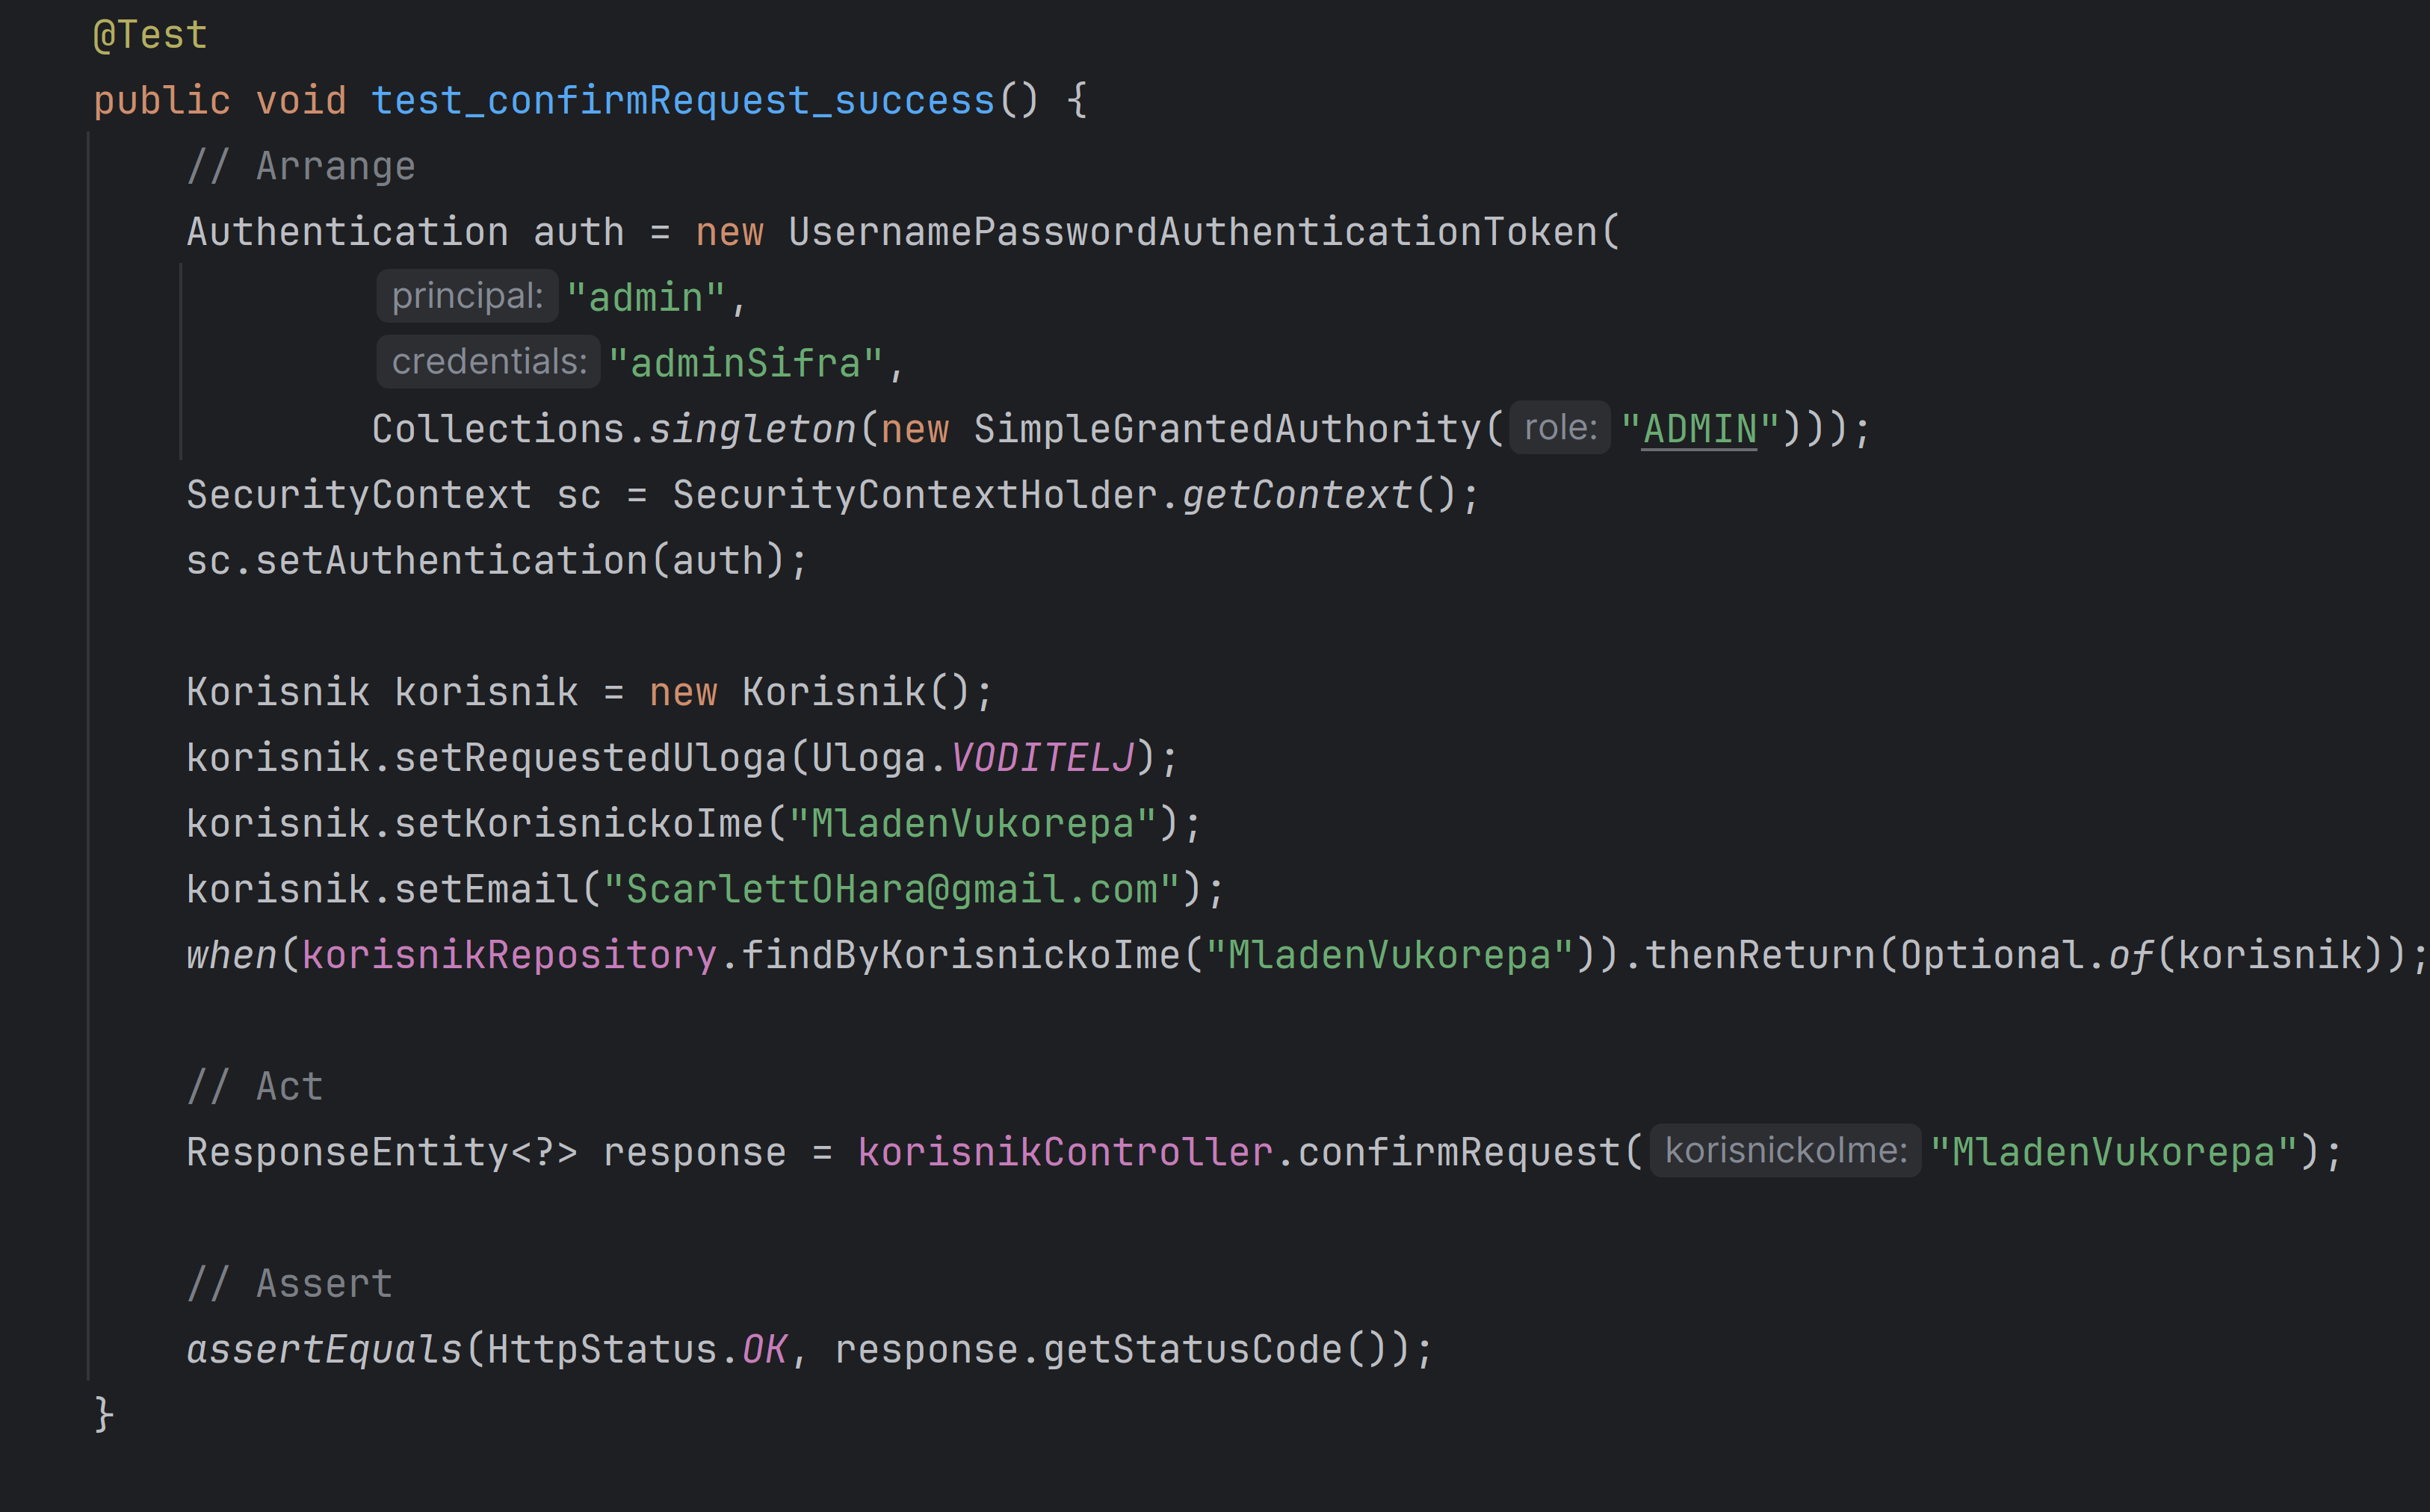
\includegraphics[scale=0.15]{slike/test3.png}
	\centering
	\caption{Testirajuća metoda - potvrda zatražene uloge}
	\label{fig:test3}
\end{figure}

S ciljem testiranja klase \textit{NatjecanjeController} napisana su dva testa. Testirajućom metodom 5.4 želimo provjeriti ispravnost metode za stvaranje novog natjecanja kada su pruženi ispravni ulazni podaci (naziv, voditelj, početak i kraj natjecanja). Očekuje se da će nakon uspješnog stvaranja natjecanja, testirana metoda vratiti odgovarajući objekt \textit{CreateNatjecanjeDTO} koji sadrži proslijeđene ulazne podatke o novostvorenom natjecanju.

\begin{figure}[H]
	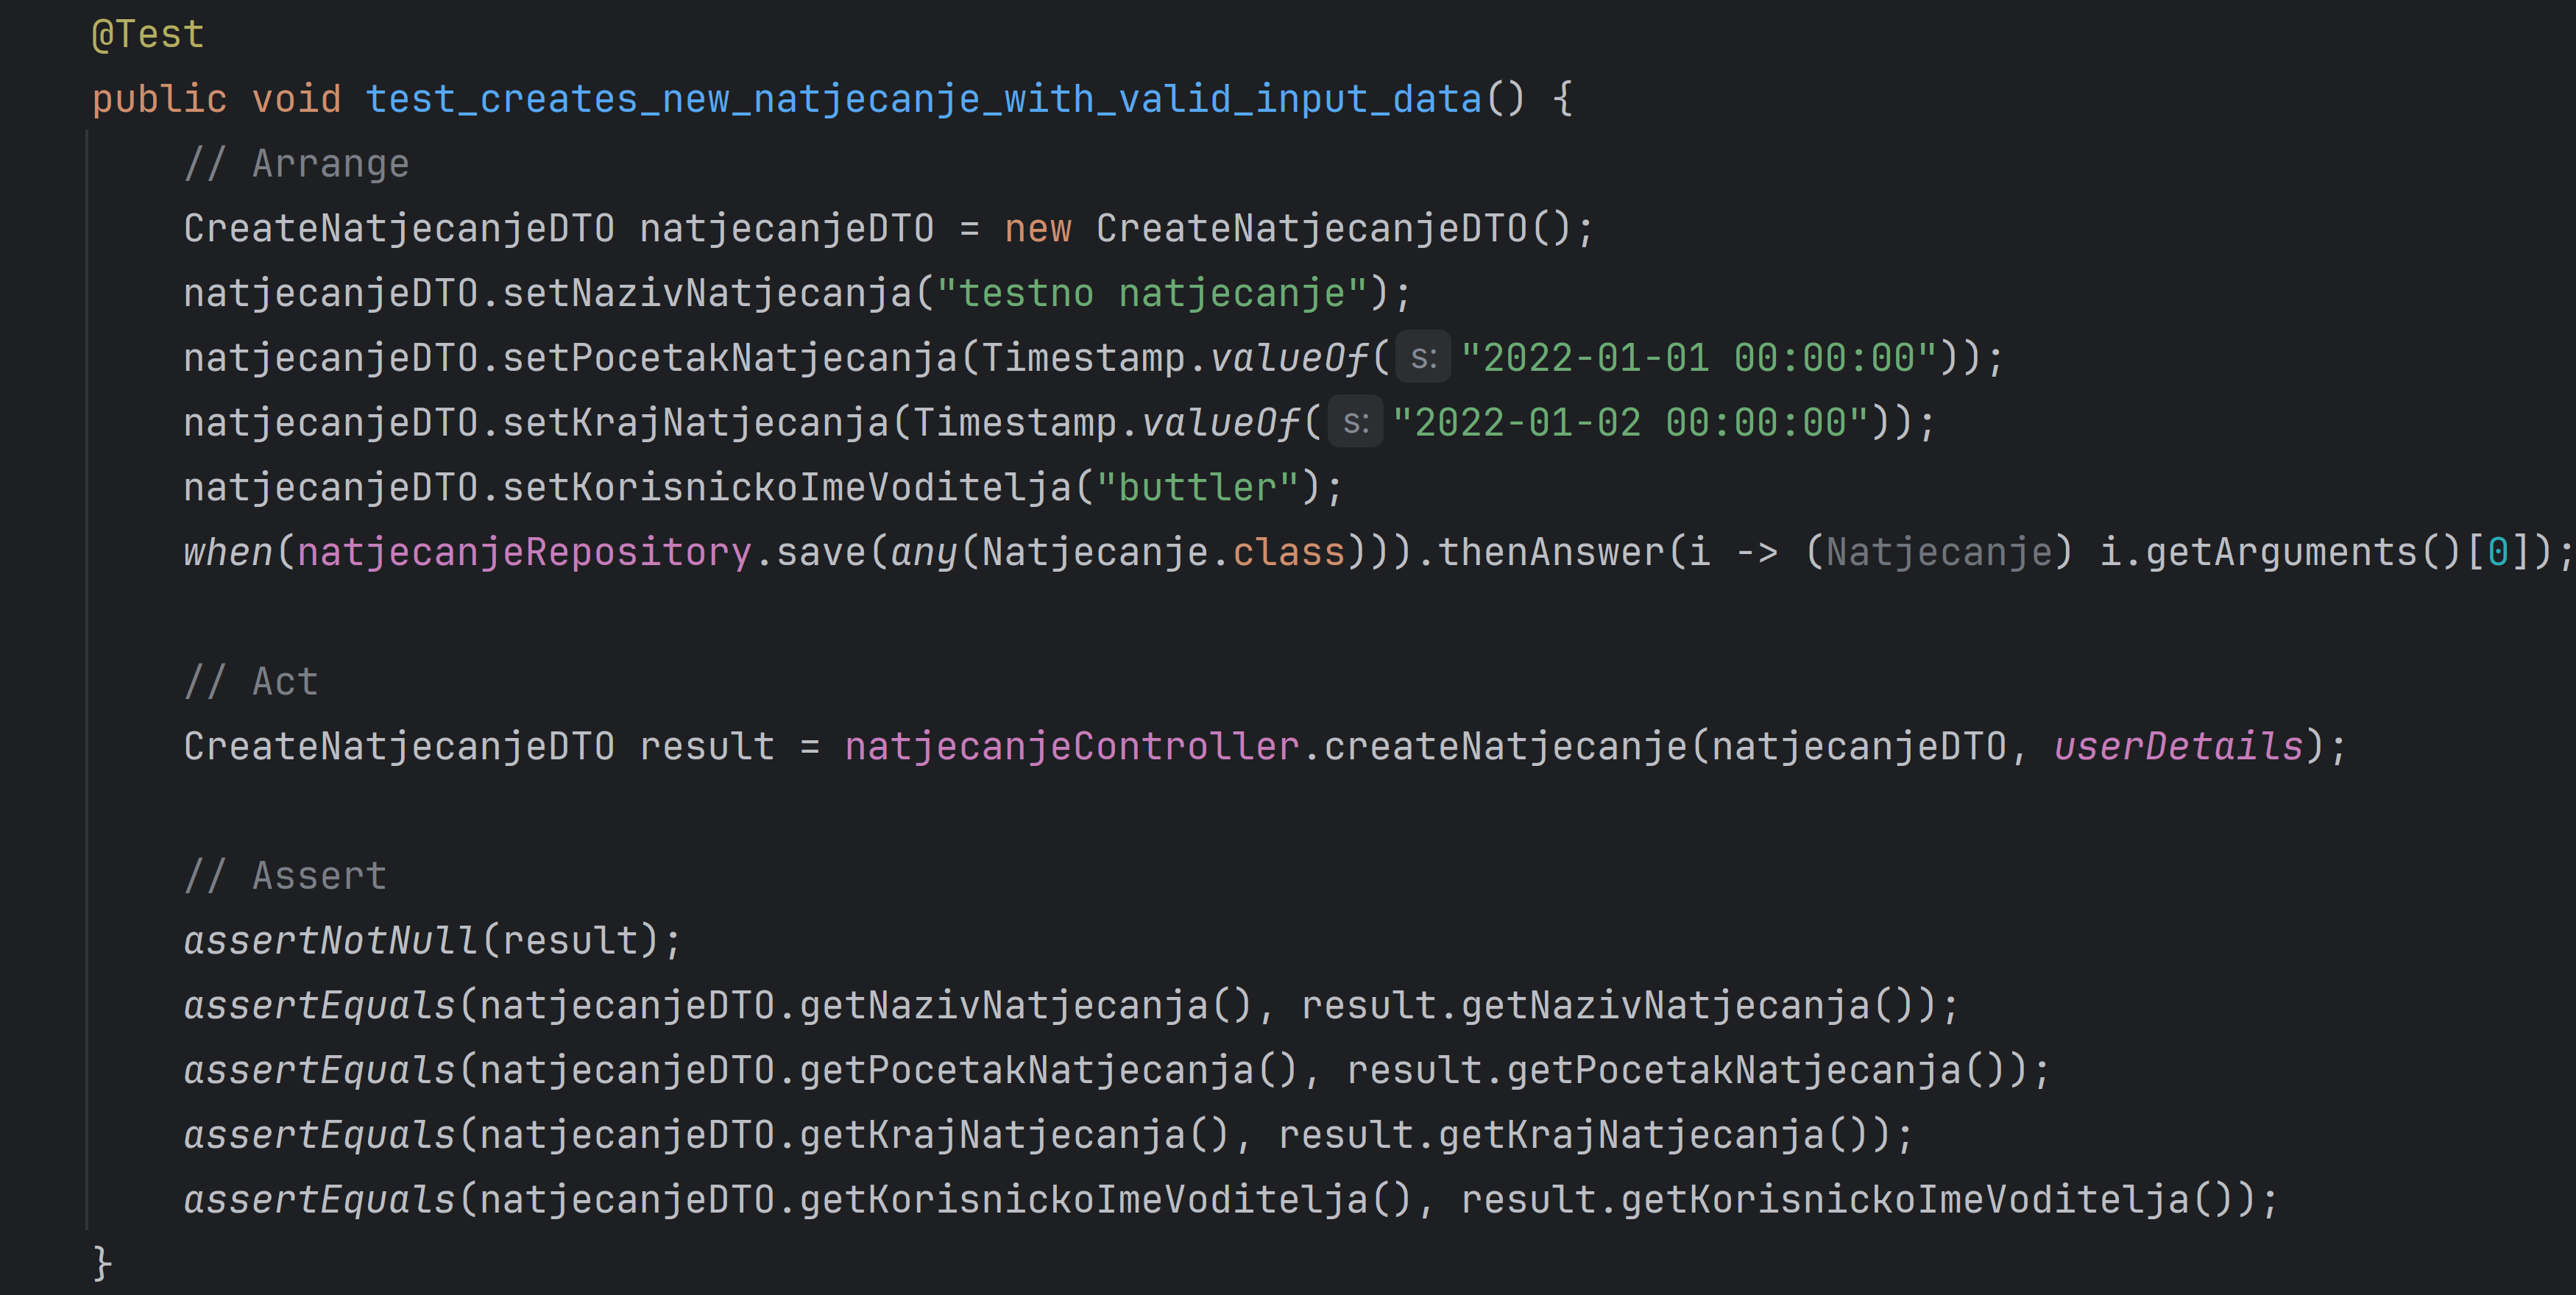
\includegraphics[scale=0.15]{slike/test4.png}
	\centering
	\caption{Testirajuća metoda - stvaranje natjecanja}
	\label{fig:test4}
\end{figure}

Druga i posljednja testirajuća metoda \ref{fig:test5} za klasu \textit{NatjecanjeController} ima za cilj provjeriti ispravnost iste metode u situaciji kada je odabrani početak natjecanja nakon završetka natjecanja. Očekuje se da će u takvim slučajevima metoda baciti iznimku.

\begin{figure}[H]
	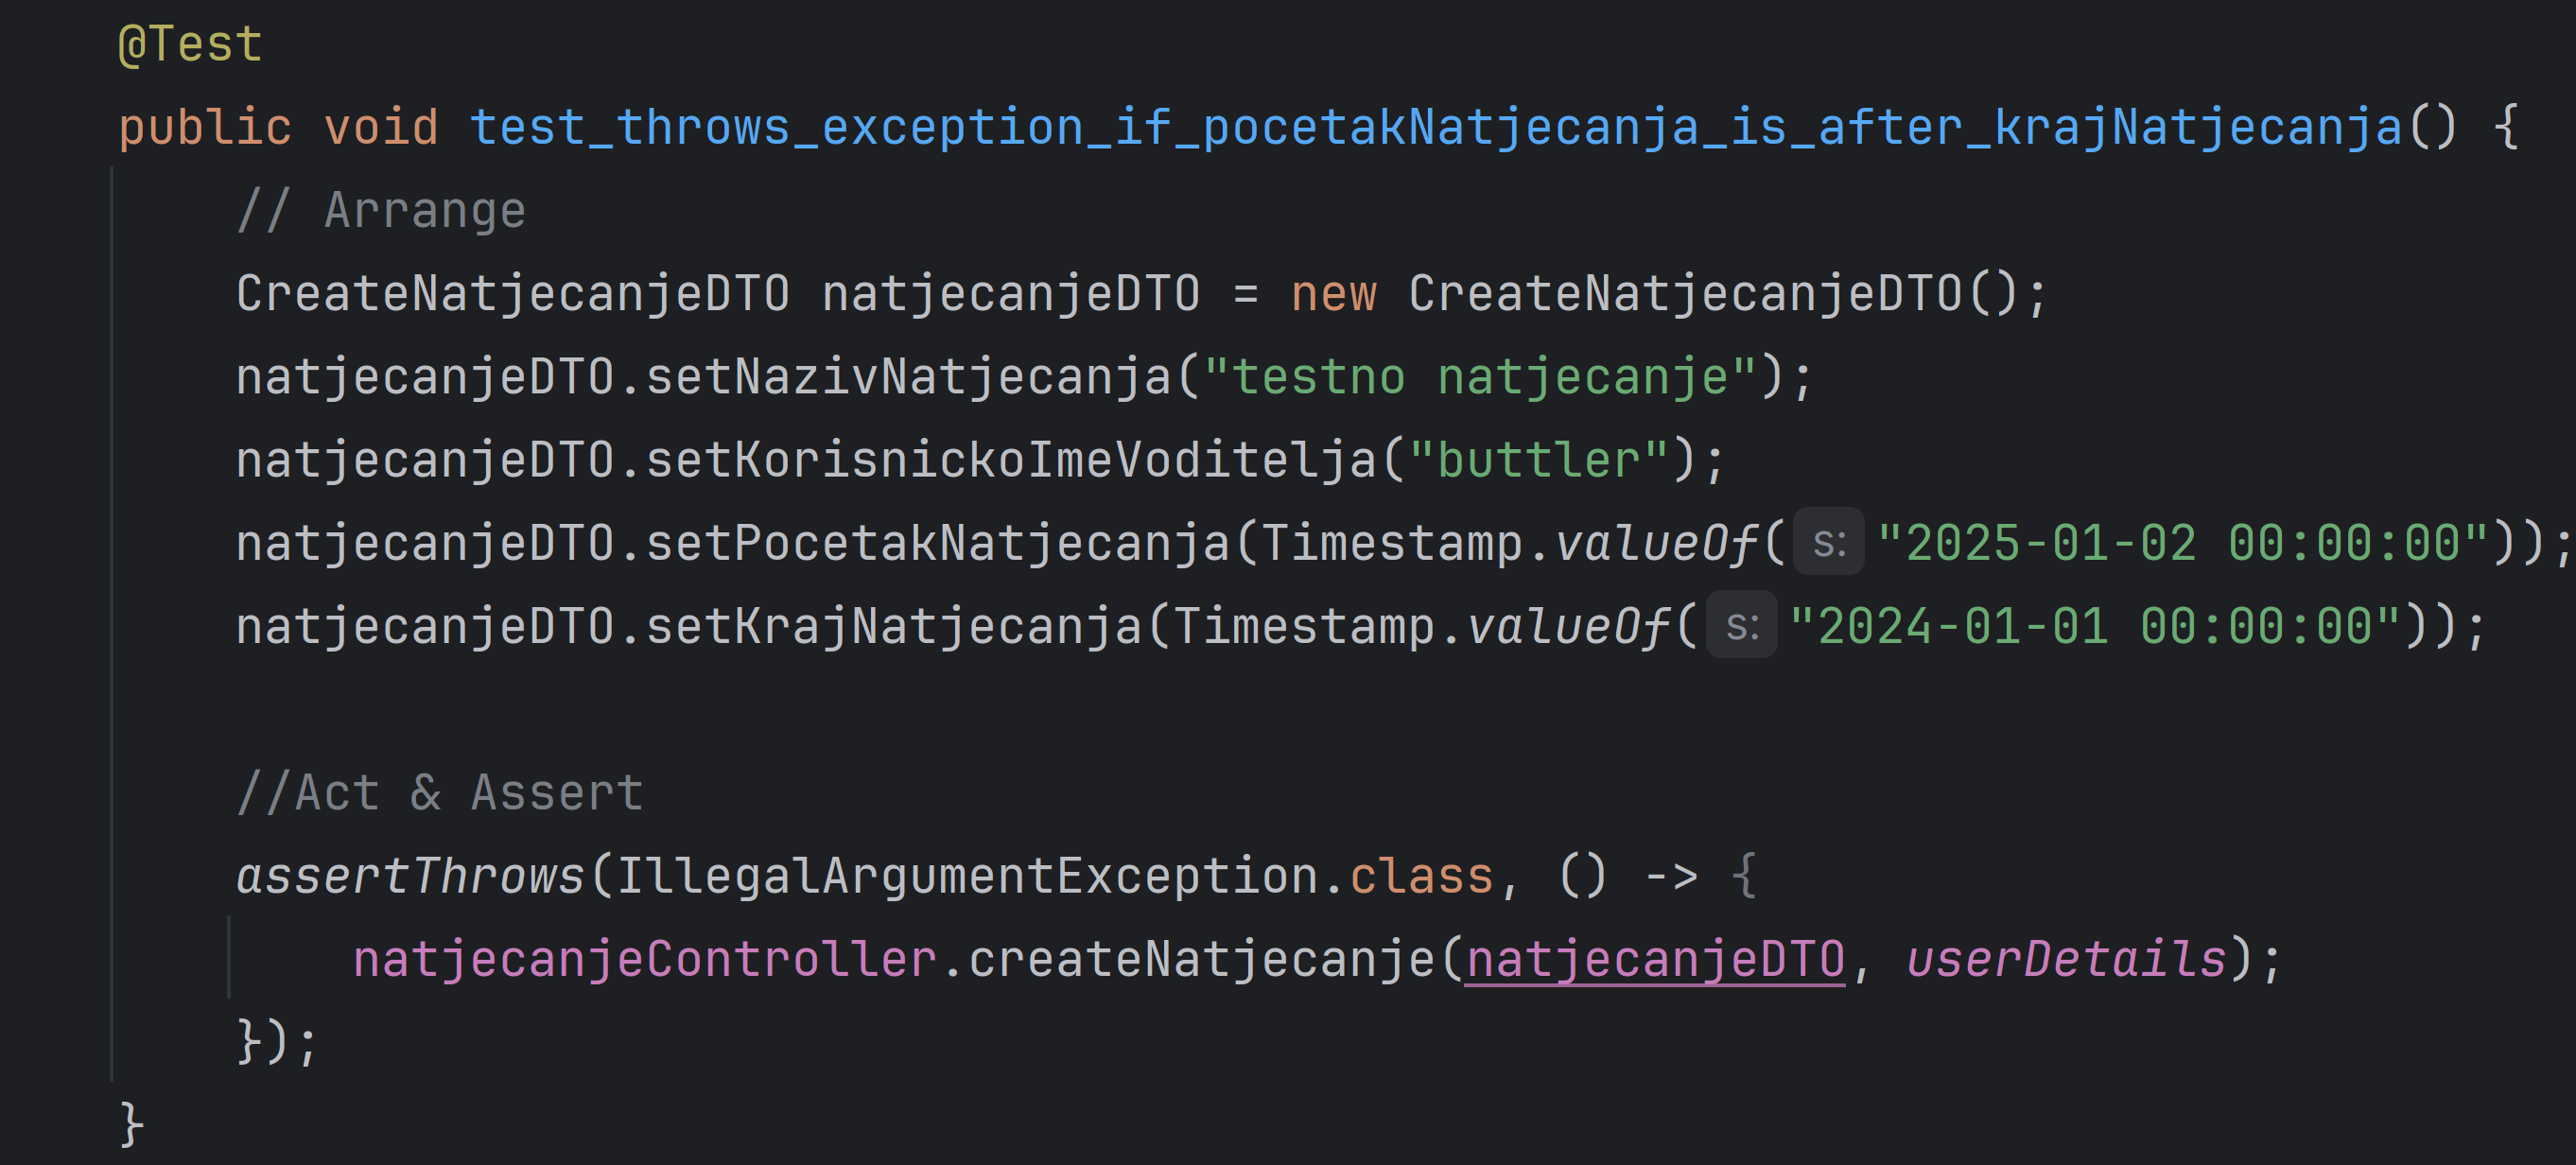
\includegraphics[scale=0.2]{slike/test5.png}
	\centering
	\caption{Testirajuća metoda - neuspješno stvaranje natjecanja}
	\label{fig:test5}
\end{figure}

Na kraju, implementirana su i dva testa za klasu \textit{ZadatakController}. U metodi \ref{fig:test6}, fokusirali smo se na testiranje metode koja dohvaća sve javne zadatke, s posebnim naglaskom na rubni slučaj kada nema dostupnih javnih zadataka. U toj situaciji očekujemo praznu listu kao povratnu vrijednost.

\begin{figure}[H]
	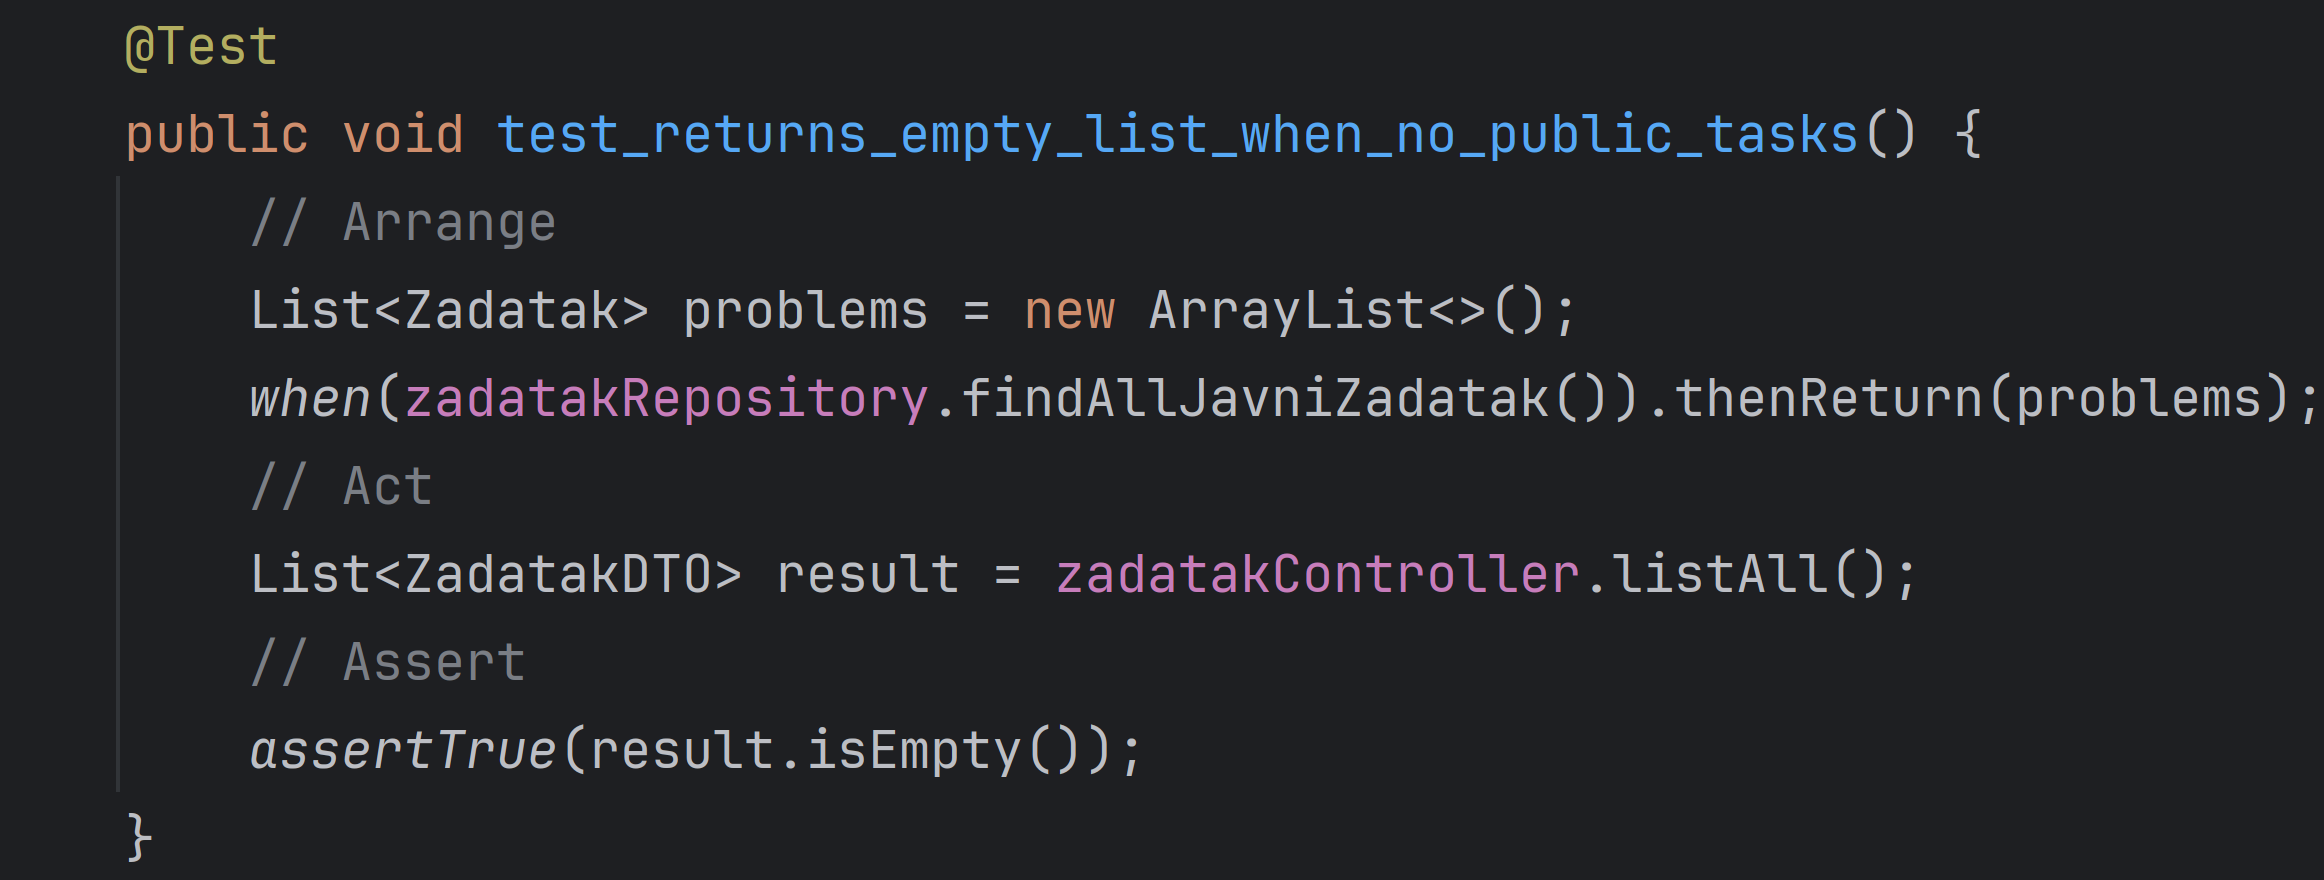
\includegraphics[scale=0.2]{slike/test6.png}
	\centering
	\caption{Testirajuća metoda - dohvat javnih zadataka}
	\label{fig:test6}
\end{figure}

Posljednjom testirajućom metodom \ref{fig:test7} ispitujemo funkcionalnost metode za ažuriranje zadatka u scenariju kada administrator želi izvršiti ažuriranje. Testiranoj metodi \textit{updateKorisnik} prosljeđujemo identifikator zadatka, podatke koje želimo ažurirati (naziv i težina) te informacije o prijavljenom korisniku (administratoru). Očekujemo da će kao izlaz metoda vratiti ažurirani objekt tipa \textit{Zadatak} te provjeravamo jesu li naziv zadatka i težina zadatka ispravno ažurirani prema zadanim promjenama.


\begin{figure}[H]
	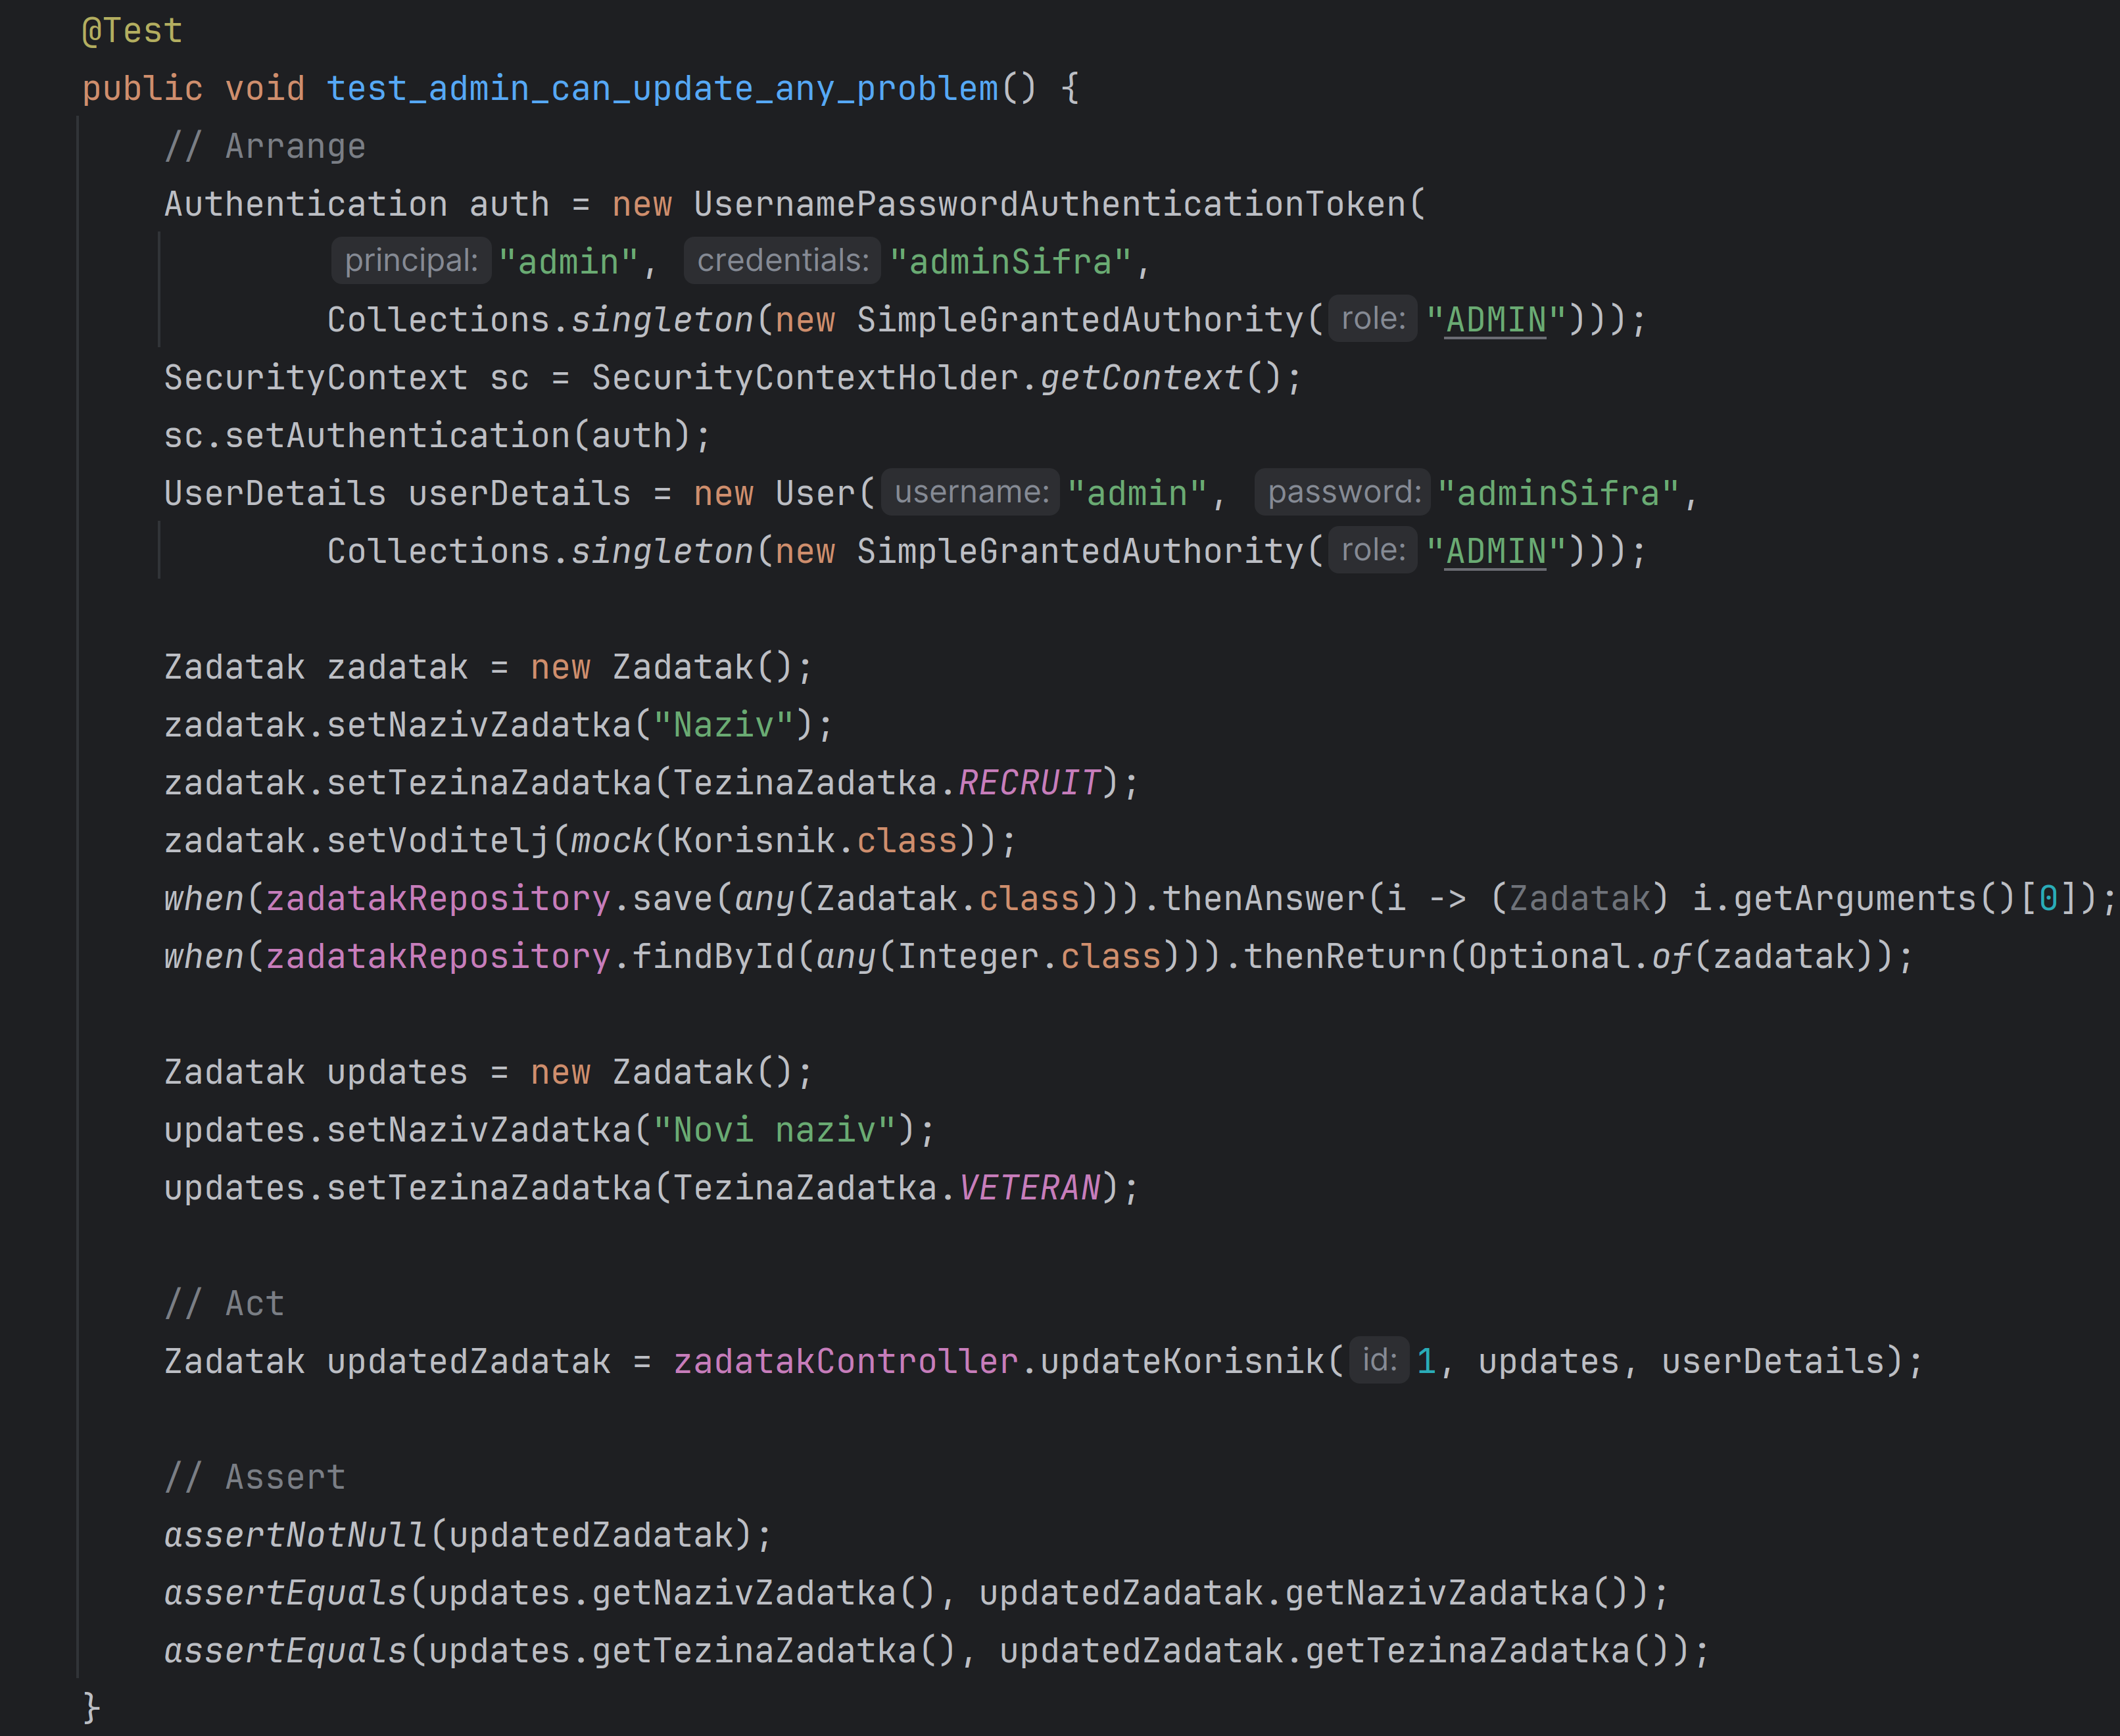
\includegraphics[scale=0.13]{slike/test7.png}
	\centering
	\caption{Testirajuća metoda - ažuriranje zadatka od strane administratora}
	\label{fig:test7}
\end{figure}

\noindent Rezultati testiranja se mogu vidjeti na slici \ref{fig:test_rezultati}.

\begin{figure}[H]
	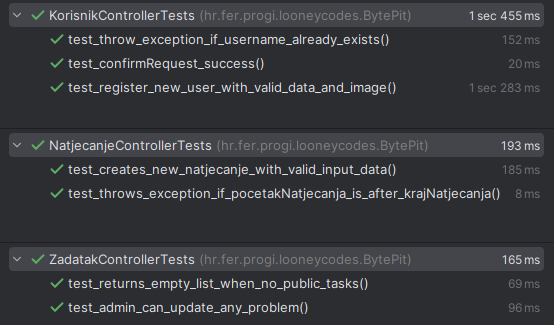
\includegraphics[scale=0.8]{slike/test_rezultati.png}
	\centering
	\caption{Rezultati testiranja}
	\label{fig:test_rezultati}
\end{figure}

\subsection{Ispitivanje sustava}

Ispitivanje sustava proveli smo pomoću \textit{Selenium Web Drivera}, implementirajući ispitne slučajeve unutar \textit{JUnit} testova. Ukupno smo napisali tri testna slučaja.

\vspace{1em}

Ispitnim slučajem \ref{fig:selenium1} ispitali smo uspješnost prijave korisnika s točnim korisničkim imenom i lozinkom te potvrdili očekivano preusmjeravanje na početnu stranicu i prisutnost gumba za odjavu.


\begin{figure}[H]
	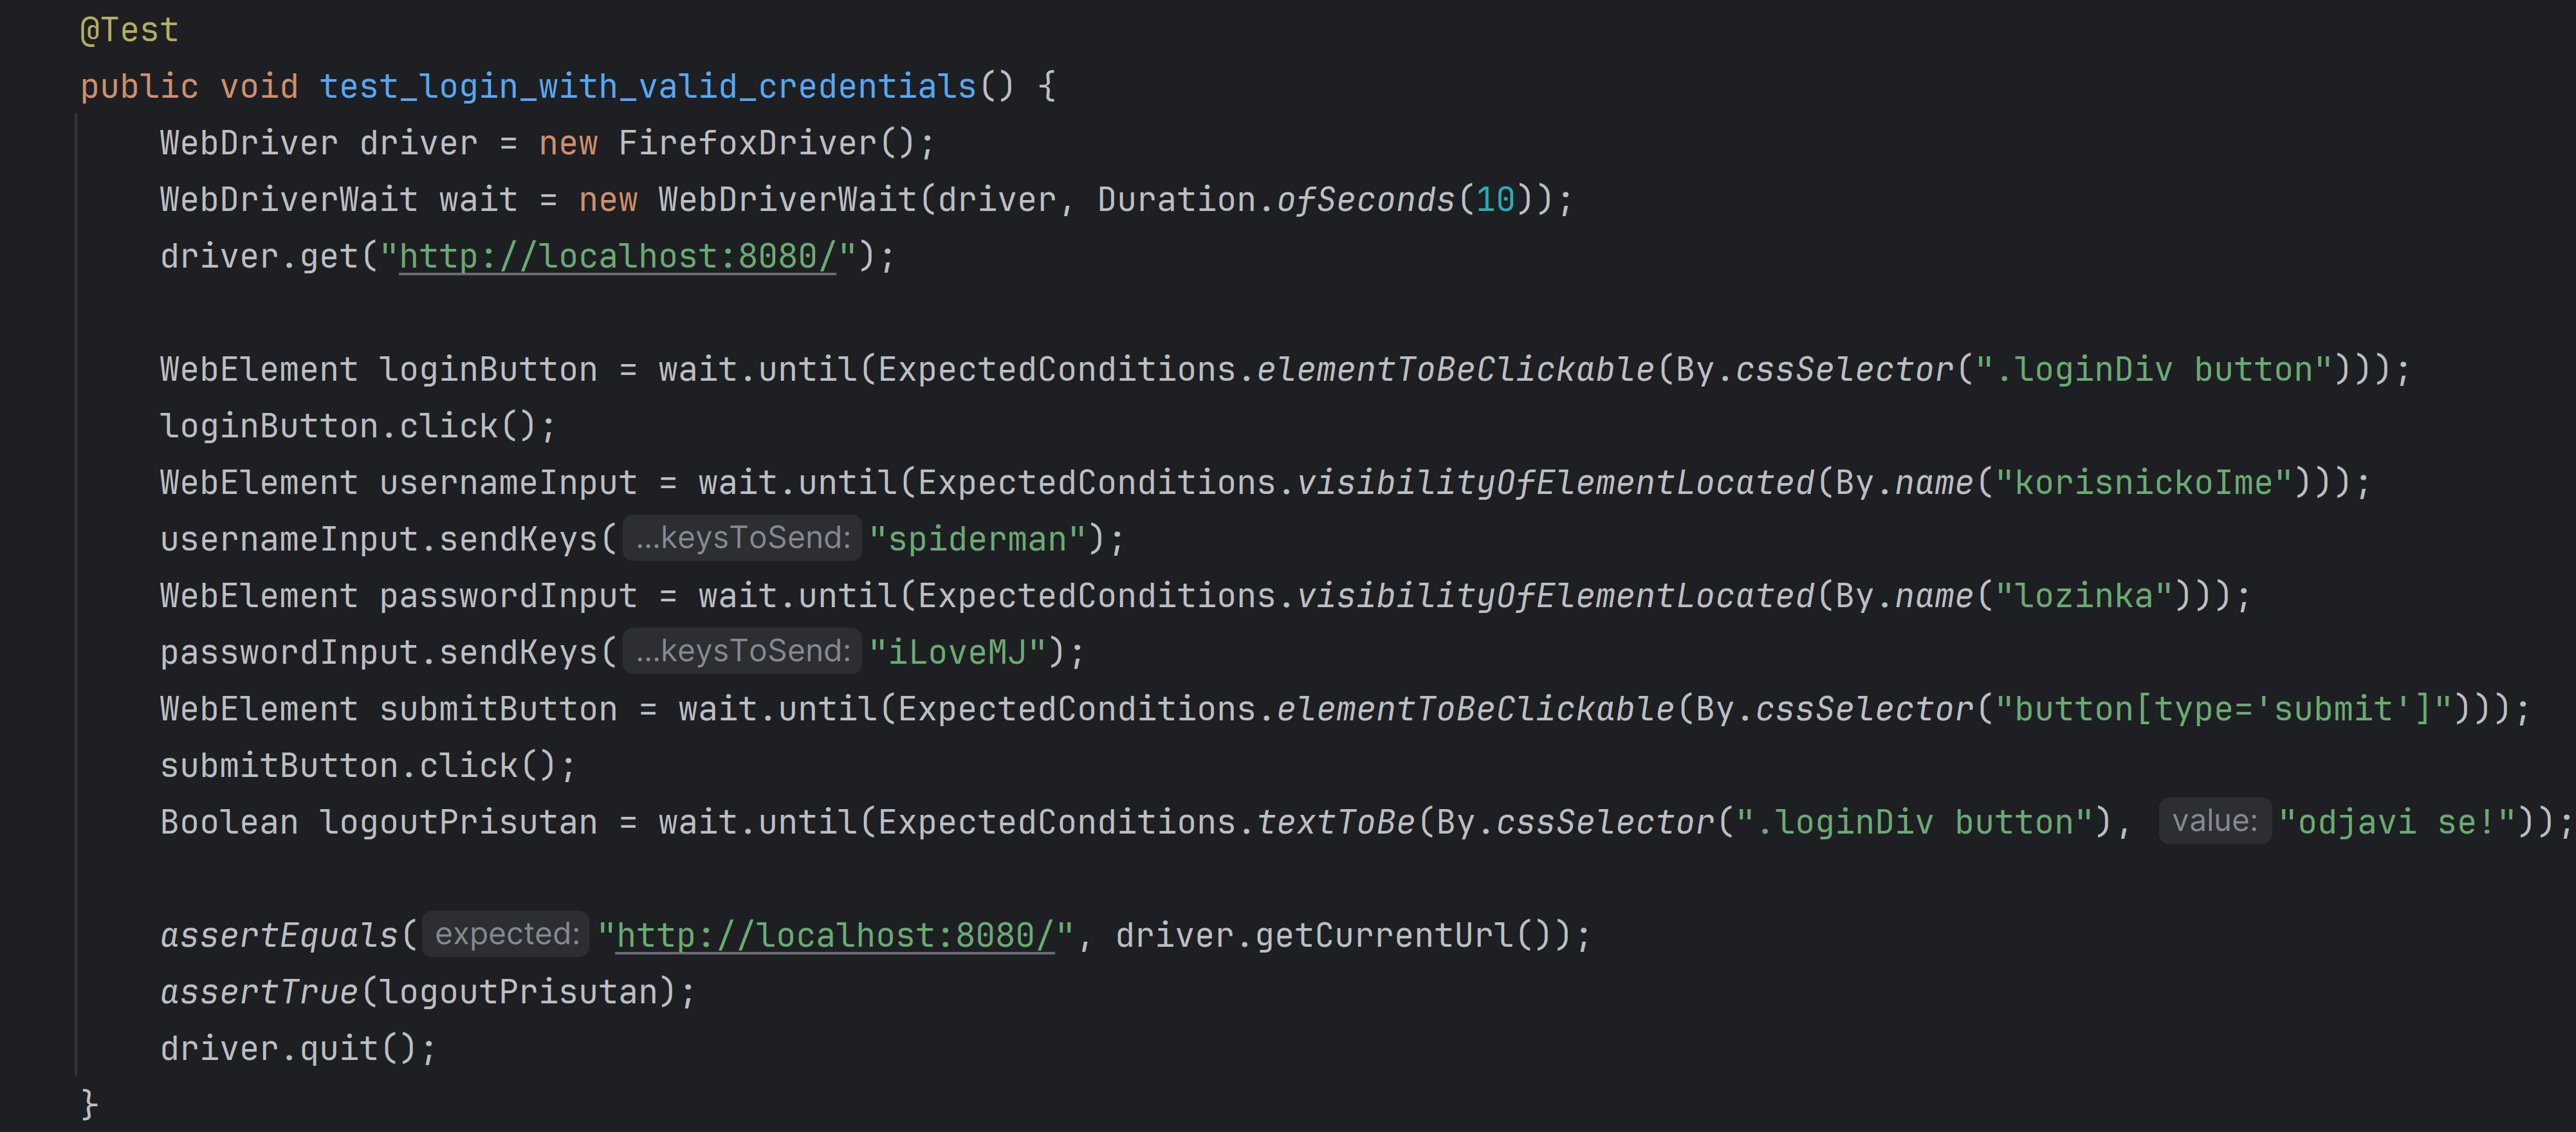
\includegraphics[scale=0.135]{slike/selenium_test1.png}
	\centering
	\caption{Selenium test - prijava korisnika s ispravnim podacima}
	\label{fig:selenium1}
\end{figure}

Testom \ref{fig:selenium2} ispitali smo ponašanje sustava prilikom pokušaja prijave s nepostojećim korisničkim imenom i lozinkom. U takvim slučajevima očekujemo zadržavanje na stranici za prijavu.

\begin{figure}[H]
	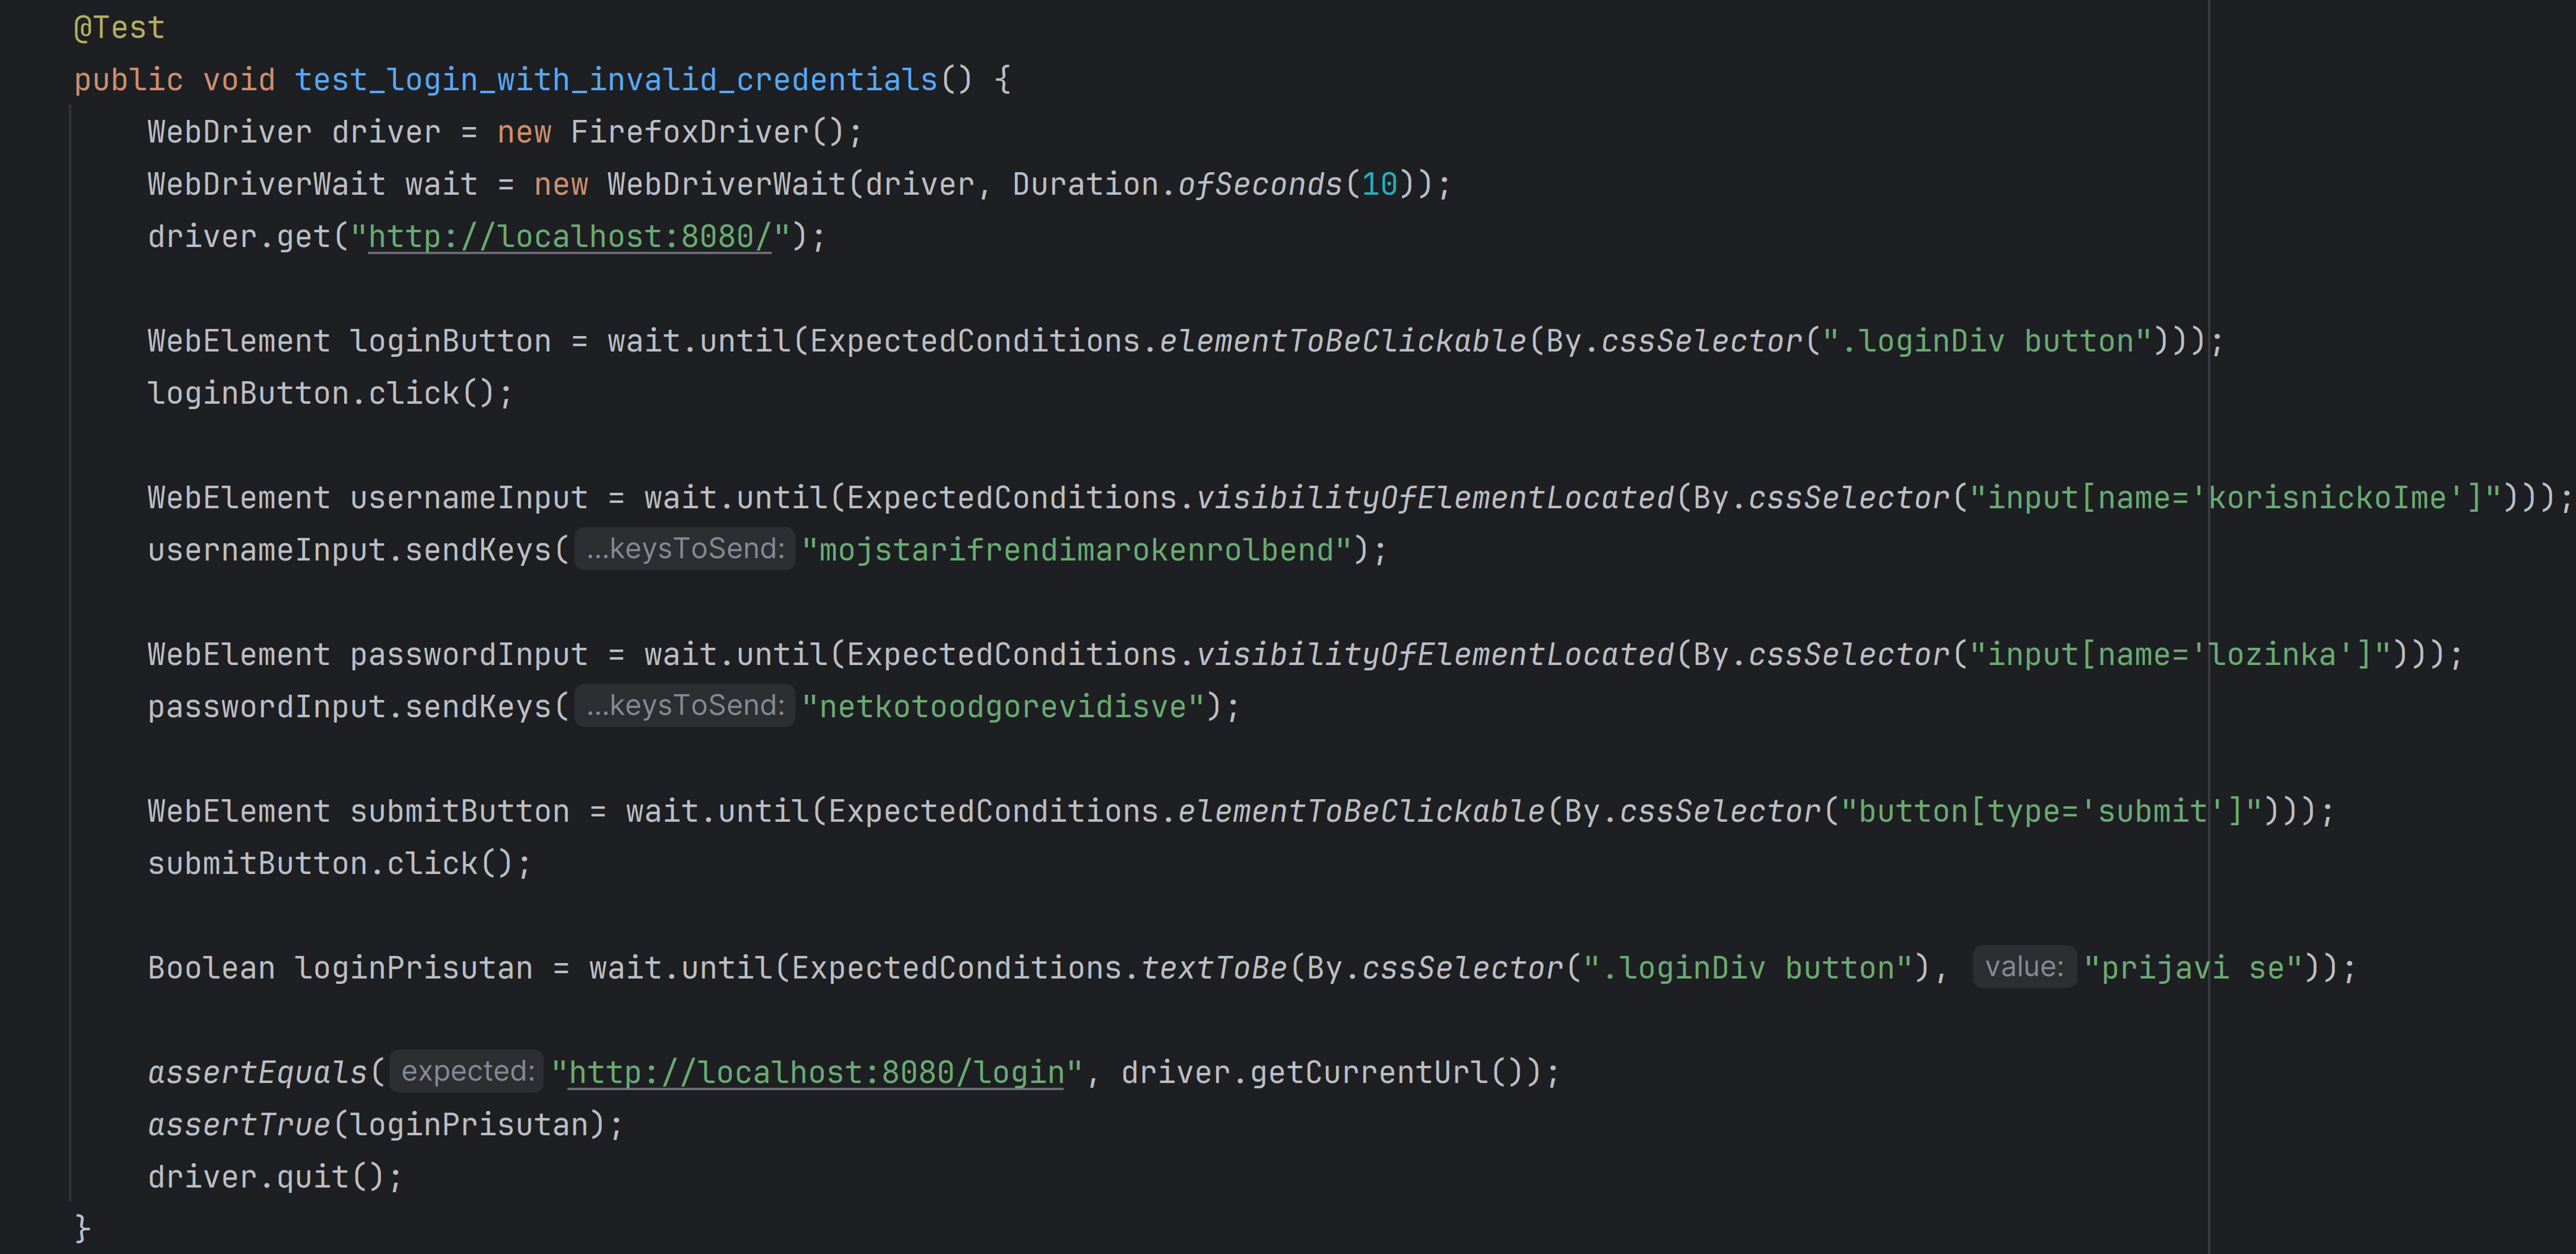
\includegraphics[scale=0.14]{slike/selenium_test2.png}
	\centering
	\caption{Selenium test - pokušaj prijave nepostojećeg korisnika}
	\label{fig:selenium2}
\end{figure}
\pagebreak
Ispitni slučaj \ref{fig:selenium3} provjerava ispravnost stvaranja novog zadatka od strane prijavljenog voditelja. Kao rezultat očekujemo pojavljivanje novostvorenog zadatka na korisničkom profilu voditelja.

\begin{figure}[H]
	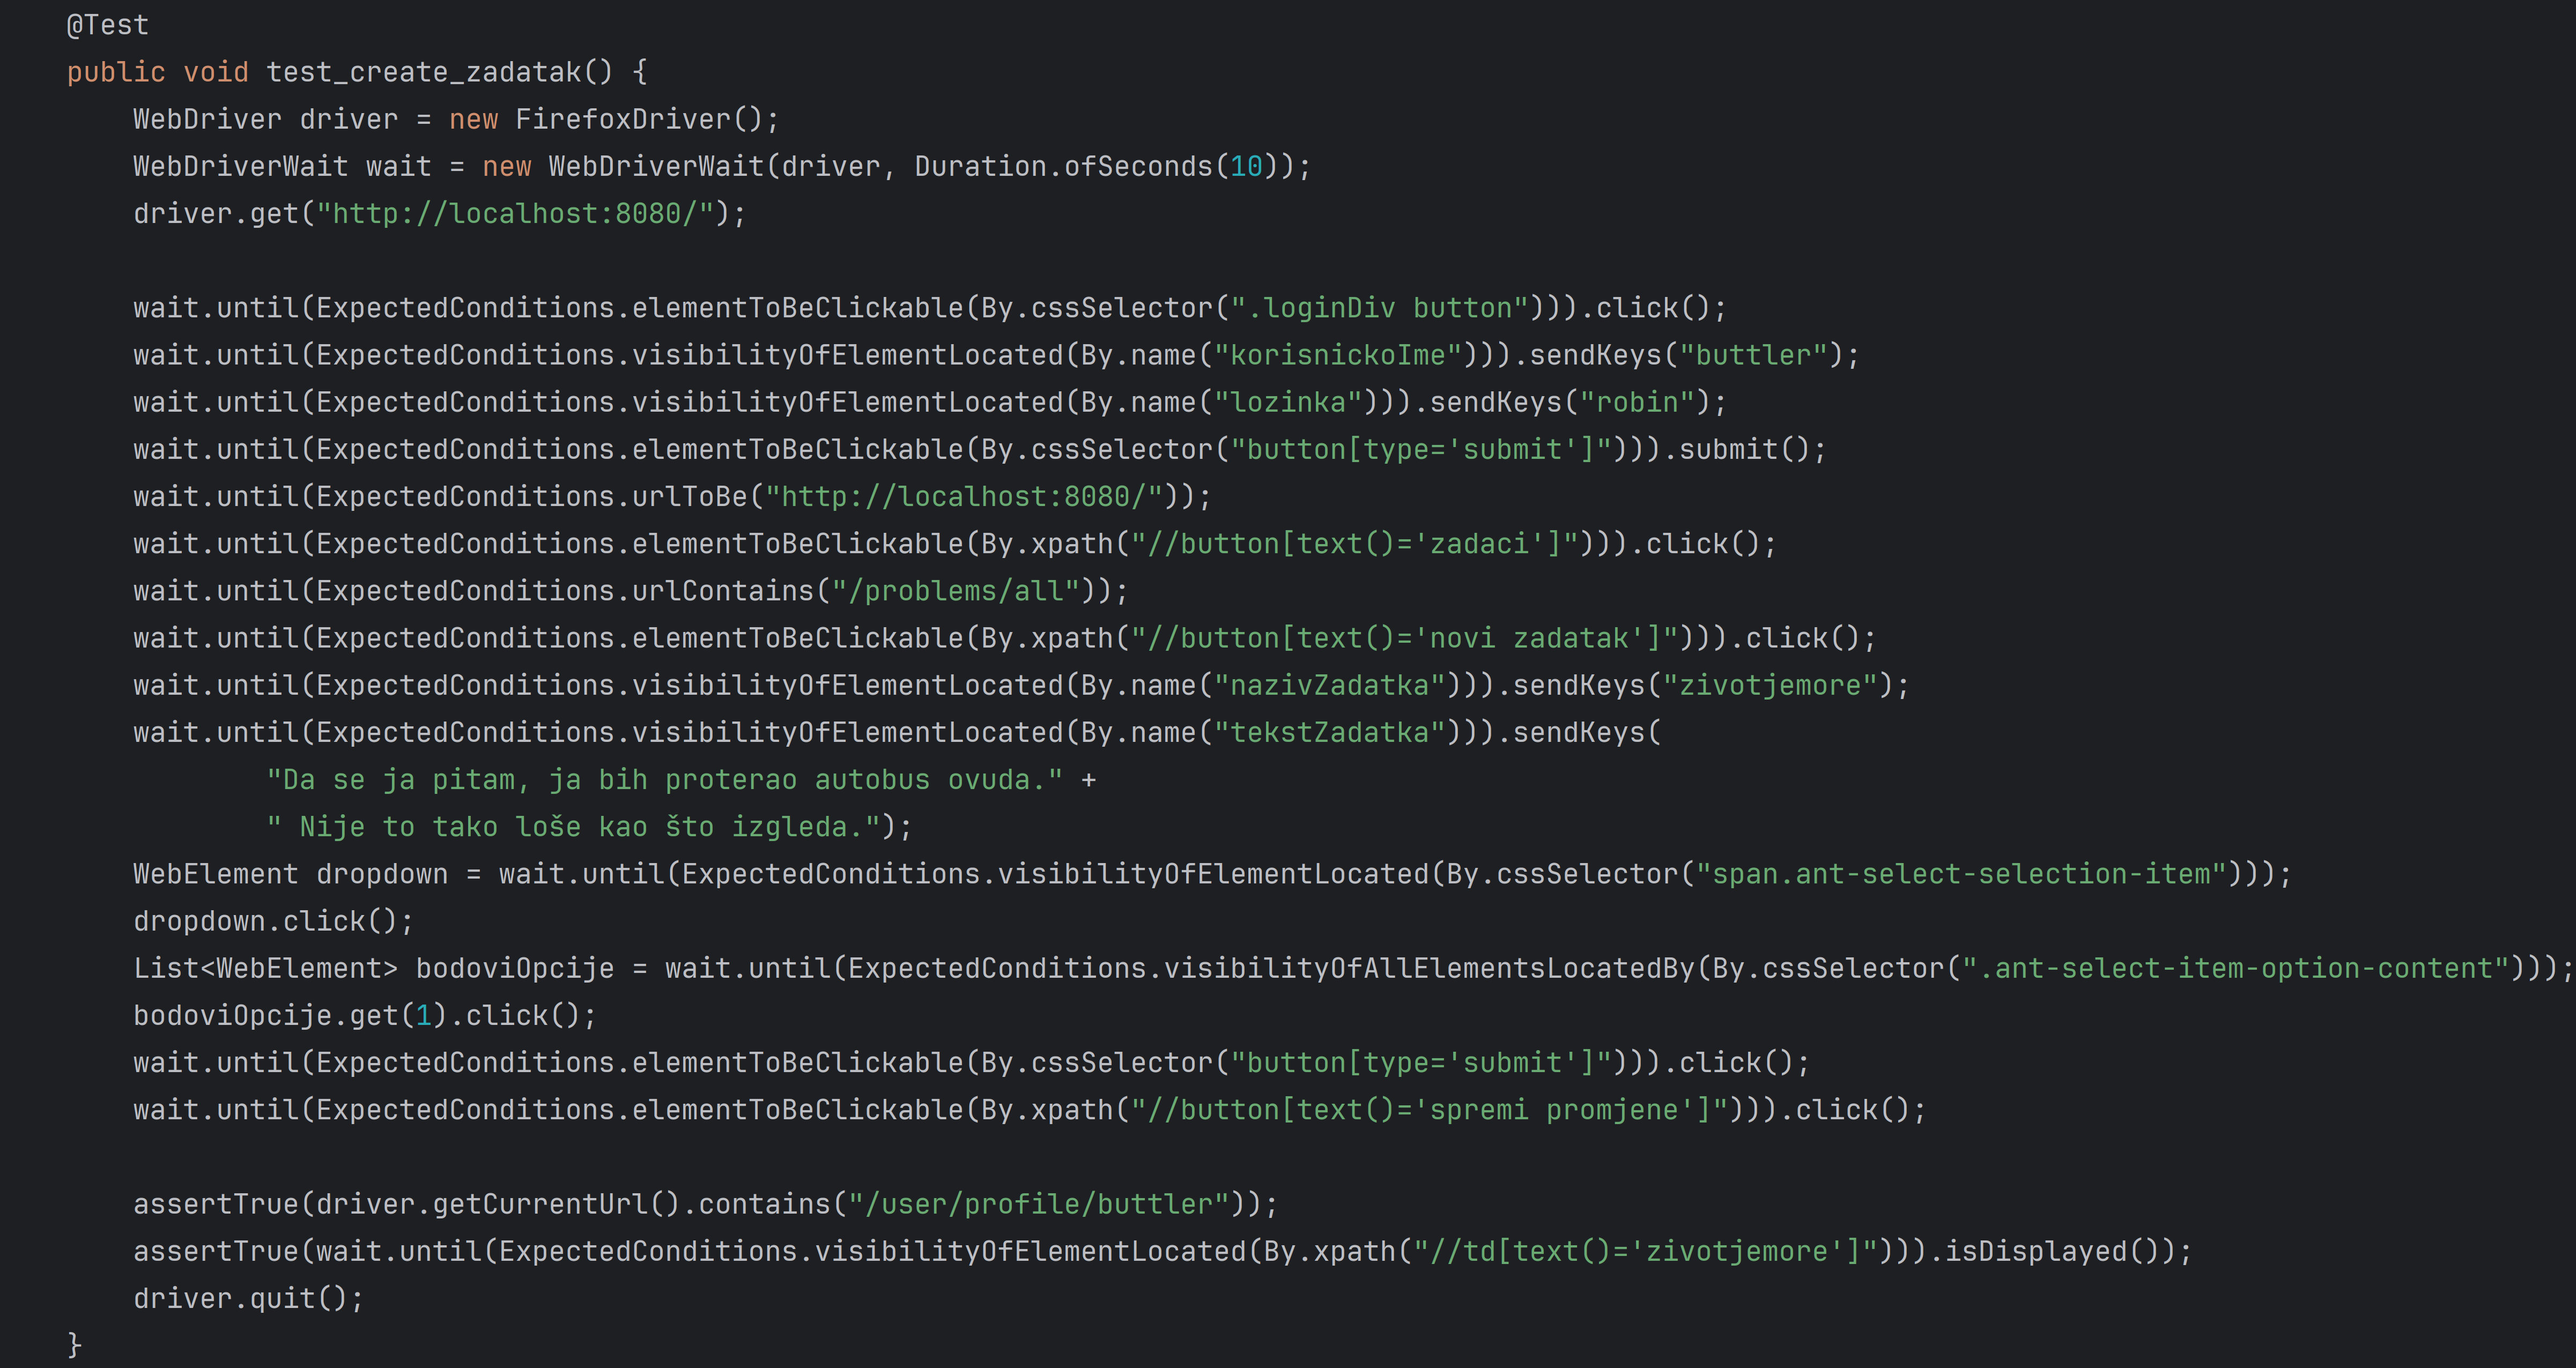
\includegraphics[scale=0.13]{slike/selenium_test3.png}
	\centering
	\caption{Selenium test - dodavanje novog zadatka}
	\label{fig:selenium3}
\end{figure}

\noindent Rezultati ispitivanja sustava mogu se vidjeti na slici \ref{fig:selenium_rezultati}.

\begin{figure}[H]
	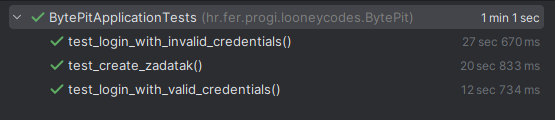
\includegraphics[scale=0.8]{slike/selenium_reultati.png}
	\centering
	\caption{Rezultati testiranja}
	\label{fig:selenium_rezultati}
\end{figure}


%\textit{Izradu ispitnih slučajeva pomoću radnog okvira Selenium moguće je provesti pomoću jednog od sljedeća dva alata:}
%\begin{itemize}
%	\item \textit{dodatak za preglednik \textbf{Selenium IDE} - snimanje korisnikovih akcija radi automatskog ponavljanja ispita	}
%	\item \textit{\textbf{Selenium WebDriver} - podrška za pisanje ispita u jezicima Java, C\#, PHP koristeći posebno programsko sučelje.}
%\end{itemize}
%\textit{Detalji o korištenju alata Selenium bit će prikazani na posebnom predavanju tijekom semestra.}

\eject



\section{Dijagram razmještaja}

UML-dijagrami razmještaja prikazuju fizičku arhitekturu i konfiguraciju razmještaja programskog sustava, a pomažu u planiranju održavanja, nadogradnji sustava, identifikaciji potencijalnih uskih grla i pojedinačnih točaka kvara. U našem primjeru, na poslužiteljskom računalu nalaze se Render web poslužitelj i poslužitelj baze podataka PostgreSQL. Poslužiteljsko računalo komunicira s klijentskim računalom putem protokola HTTPS, a na klijentskom računalu pristupamo aplikaciji putem odabranog web preglednika. Osim s klijentskim računalom, poslužiteljsko računalo komunicira i sa servisom za slanje emailova Mailjet, a koristi se i API za evaluaciju programskog rješenja kojeg predaju natjecatelji Judge0.

\begin{figure}[H]
	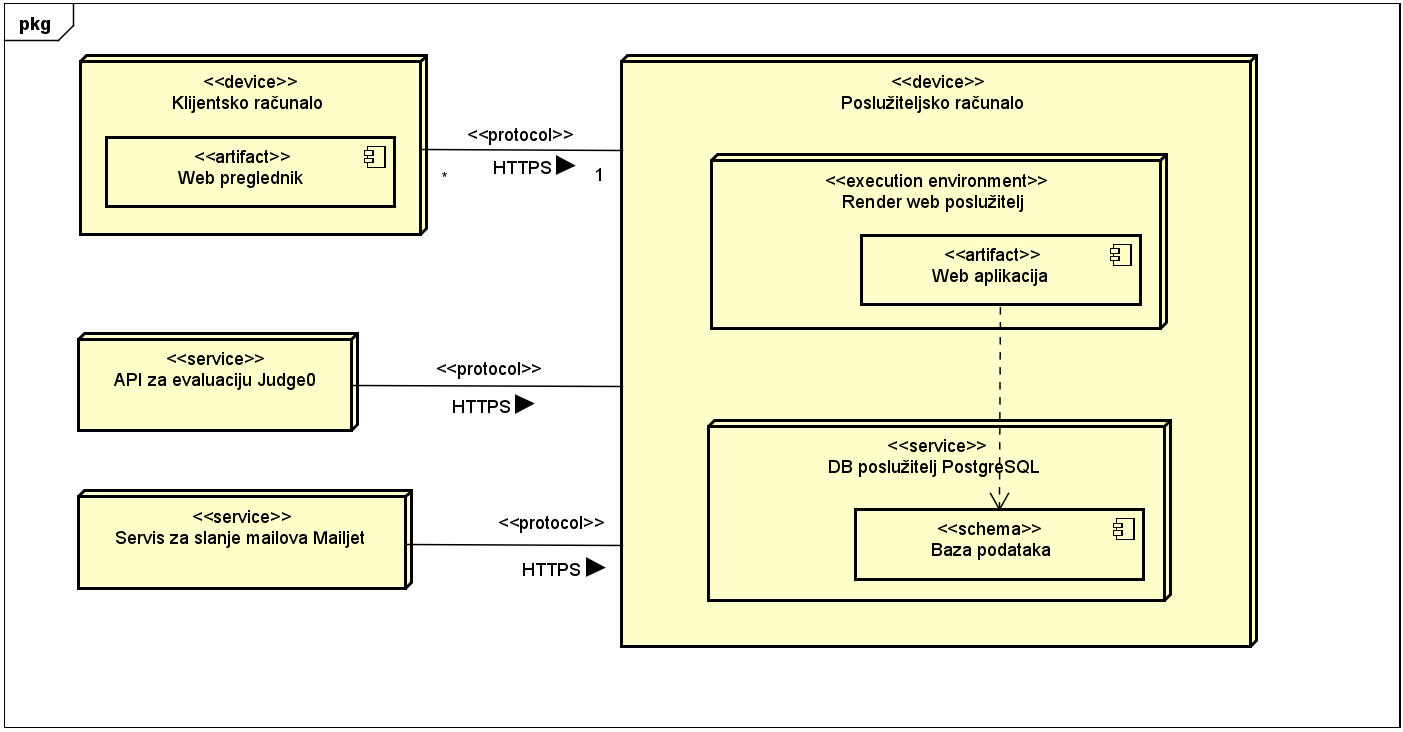
\includegraphics[scale=0.70]{dijagrami/dijagram_razmjestaja}
	\centering
	\caption{Dijagram razmještaja}
\end{figure}

\eject

\section{Upute za puštanje u pogon}

Za puštanje našeg projekta u pogon može se koristiti Render.com. Ovu smo platformu odabrali zbog njezine jednostavnosti i pristupačnosti. U nastavku ćemo opisati korake koje smo poduzeli kako bismo uspješno postavili našu aplikaciju na Render.com.


Na početku je potrebno pripremiti GitHub repozitorij i stvoriti korisnički račun na Renderu. Dovoljno je za kratkoročnu uporabu koristiti besplatni plan na obje platforme.
Aplikacija je prilagođena za korištenje izgrađenih statičkih resursa korisničke strane koji se potom dostavljaju s poslužitelja. Prije samog pokretanja u pogon potrebno je generirati te datoteke naredbom \textit{npm run build} iz vršnog foldera implementacije klijentske strane kao što je prikazano na slici dolje.

\begin{figure}[H]
	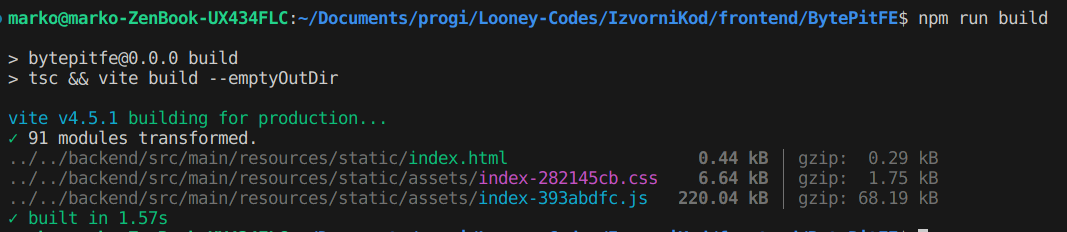
\includegraphics[scale=0.4]{slike/deployment1.png}
	\centering
	\caption{Generiranje statičkih resursa korisničke strane}
	\label{deployment1}
\end{figure}


Prije postavljanja na GitHub potrebno je napraviti Maven Wrapper naredbom \textit{mvn wrapper:wrapper} u vršnom direktoriju izvornog koda poslužiteljske strane te dodati u isti direktorij direktorij naziva \textit{Docker} koji sadrži datoteku \textit{Dockerfile} sadržaja kao na donjoj slici. Sve spomenute datoteke valja spremiti u GitHub repozitorij zajedno s ostatkom izvornog koda. 

\begin{figure}[H]
	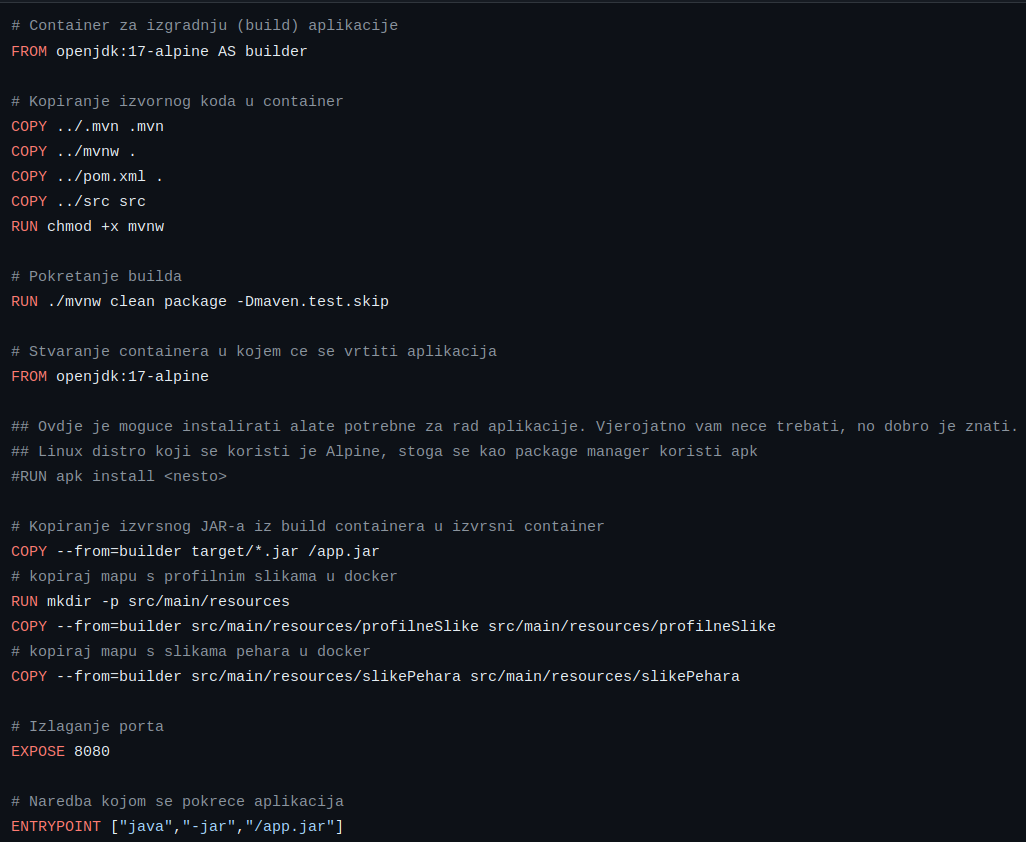
\includegraphics[scale=0.4]{slike/deployment2.png}
	\centering
	\caption{Dockerfile korišten za puštanje u pogon}
	\label{deployment2}
\end{figure}

Sada prelazimo na pokretanje aplikacije na Render platformi. Koraci koje treba obaviti su: 

\begin{itemize}
	\item \textbf{Stvaranje baze podataka} \newline
	Po izradi računa treba otvoriti novu PostgreSQL bazu podataka pritiskom na \textit{new} gumb u izborniku početne stranice i odabirom prikladne opcije. Postaviti željeno ime baze i korisnika te regiju na Frankfurt (EU Central). U \textit{application.properties} datoteci treba postaviti \textit{spring.datasource.url} na dobivenu adresu baze i \textit{spring.datasource.username} te \textit{spring.datasource.password} na dobivene korisničke podatke, a promjene pohraniti na GitHub repozitorij.
	\item \textbf{Stvaranje novog web servisa} \newline
	Slijedi inicijalizacija novog web servisa za poslužitelj naše stranice. Odabir početka stvaranja takvog servisa vrši se na sličan način kao i stvaranje nove baze podataka - pritiskom \textit{new} gumb u izborniku početne stranice i odabirom prikladne opcije.  \newline
	Pri početnom odabiru odabrati \textit{Build and deploy from a Git repository} te zatim povezati sa željenim GitHub repozitorijem. Na slici \ref{deployment3} prikazan je odabir vršnog direktorija i grane repozitorija. Kao \textit{Environment} odabrati Docker, a vrijednost putanje do \textit{Dockerfilea} treba biti postavljena na \textit{./Docker/Dockerfile}. Nije potrebno postavljati varijable okruženja jer su postavljene u aplikacijskim specifikacijama. Završiti kreiranje novog web servisa pritiskom na gumb \textit{Create Web Service}.
	\begin{figure}[H]
		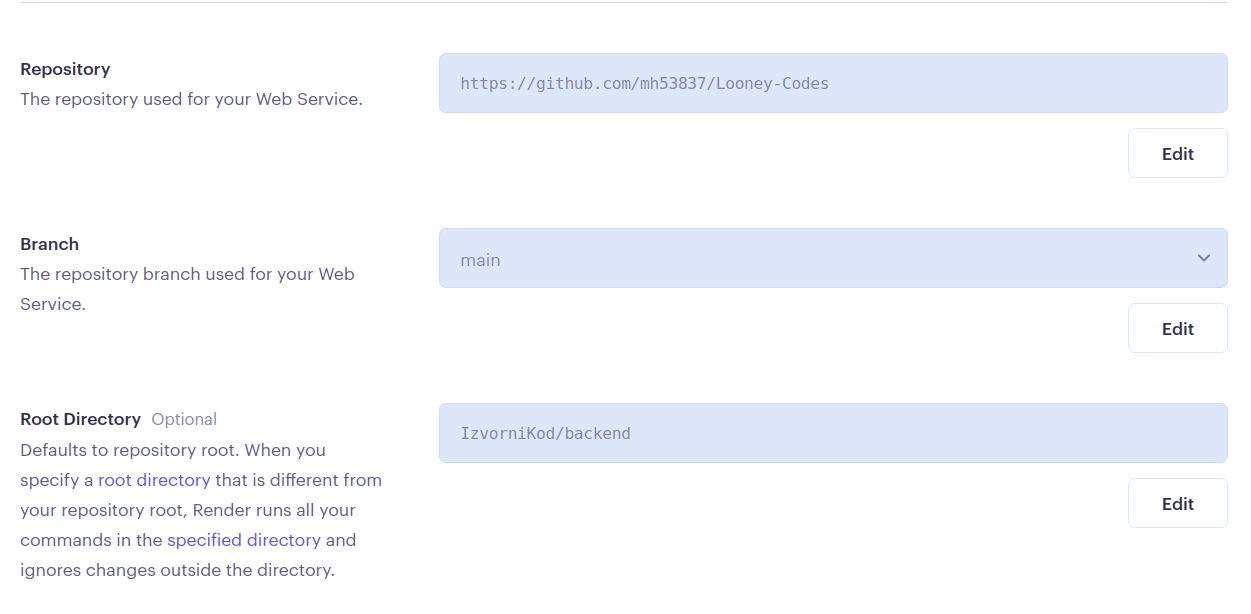
\includegraphics[scale=0.3]{slike/deployment3.png}
		\centering
		\caption{Povezivanje s GitHub repozitorijem}
		\label{deployment3}
	\end{figure}
	\item \textbf{Pokretanje web servisa}
	Po stvaranju web servisa počet će proces inicijalizacije poslužitelja. Prilikom toga na karticama \textit{Events} i \textit{Logs} potrebno je pratiti uspješnost puštanja u pogon kako bi se uvidjeli eventualni problemi i ispravili isti (ako pažljivo nije proveden neki od prethodnih koraka treba se vratiti i ponoviti ga). U logovima moguće je vidjeti kako se prvo vrši alociranje samog poslužitelja, pa \textit{dokerizacija} i na kraju se pokreće naša aplikacija. Kada je završeno puštanje u pogon moguće je vidjeti obavijest kao na slici ispod.
	\begin{figure}[H]
		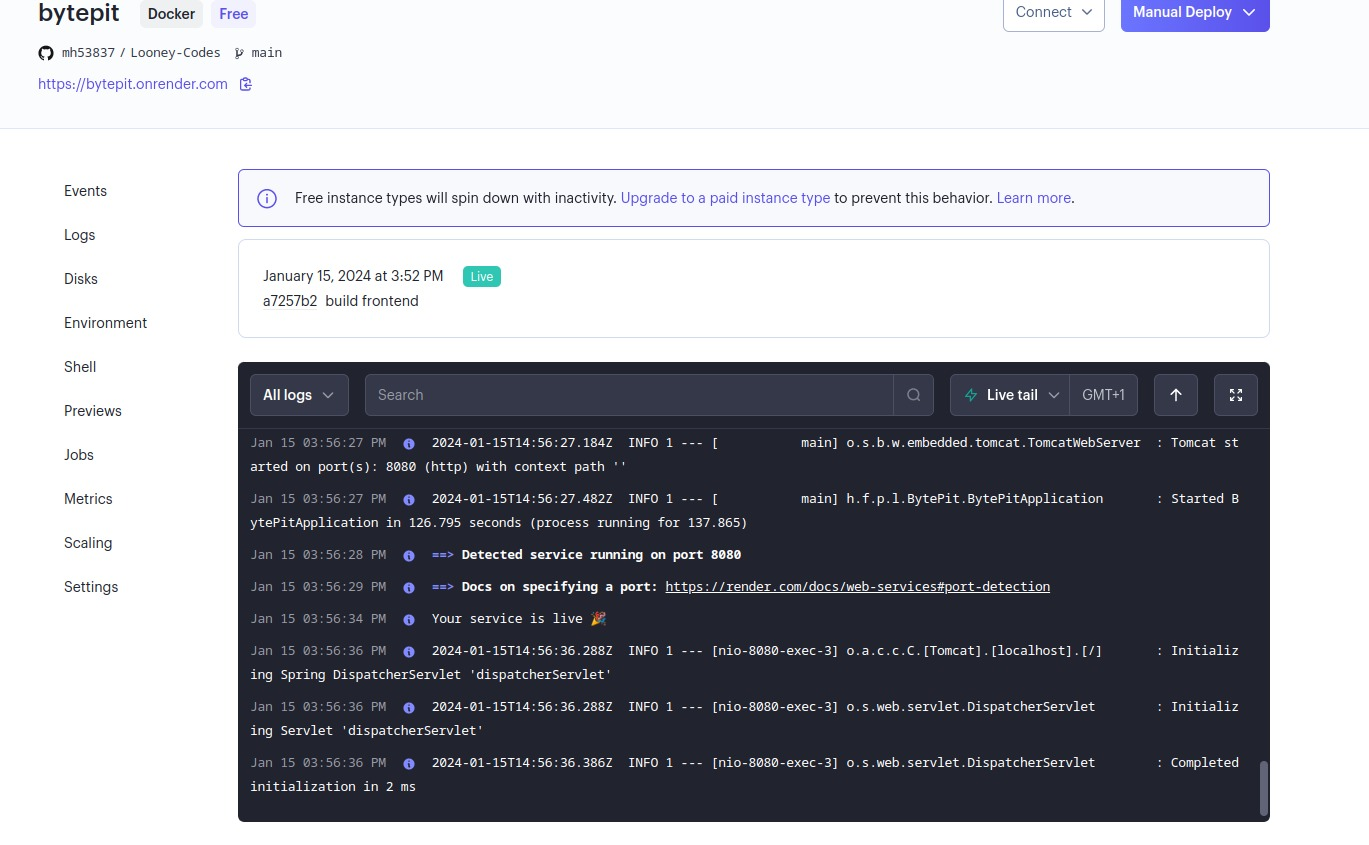
\includegraphics[scale=0.3]{slike/deployment4.jpeg}
		\centering
		\caption{Završetak pokretanja web servisa}
		\label{deployment4}
	\end{figure}
\end{itemize}

Nakon završetka puštanja u pogon na Renderu, moguće se spojiti na bazu s prije-dobivenim korisničkim podacima. Ovo je moguće napraviti kroz grafičko sučelje (primjerice PGAdmin) ili kroz naredbenu liniju. Po spajanju se dolje prikazanom naredbom u bazu podataka mogu dodati inicijalni korisnici i primjeri ostalih entiteta.

\begin{figure}[H]
	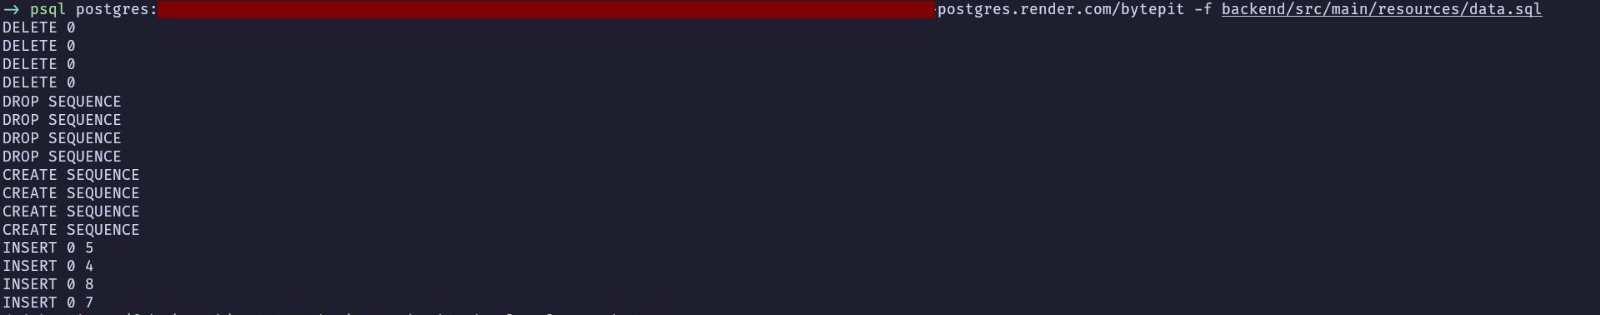
\includegraphics[scale=0.25]{slike/deployment5.jpeg}
	\centering
	\caption{Dodavanje podataka u bazu}
	\label{deployment5}
\end{figure}

Primjer naše aplikacije moguće je pronaći na poveznici \href{https://bytepit.onrender.com/}{bytepit.onrender.com}. 


\eject 